%%%%%%%%%%%%%%%%%%%%%%% file template.tex %%%%%%%%%%%%%%%%%%%%%%%%%
%
% This is a general template file for the LaTeX package SVJour3
% for Springer journals.          Springer Heidelberg 2010/09/16
%
% Copy it to a new file with a new name and use it as the basis
% for your article. Delete % signs as needed.
%
% This template includes a few options for different layouts and
% content for various journals. Please consult a previous issue of
% your journal as needed.
%
%%%%%%%%%%%%%%%%%%%%%%%%%%%%%%%%%%%%%%%%%%%%%%%%%%%%%%%%%%%%%%%%%%%
%
% First comes an example EPS file -- just ignore it and
% proceed on the \documentclass line
% your LaTeX will extract the file if required
\begin{filecontents*}{example.eps}
%!PS-Adobe-3.0 EPSF-3.0
%%BoundingBox: 19 19 221 221
%%CreationDate: Mon Sep 29 1997
%%Creator: programmed by hand (JK)
%%EndComments
gsave
newpath
  20 20 moveto
  20 220 lineto
  220 220 lineto
  220 20 lineto
closepath
2 setlinewidth
gsave
  .4 setgray fill
grestore
stroke
grestore
\end{filecontents*}
%
\RequirePackage{fix-cm}
%
%\documentclass{svjour3}                     % onecolumn (standard format)
%\documentclass[smallcondensed]{svjour3}     % onecolumn (ditto)
\documentclass[smallextended]{svjour3}       % onecolumn (second format)
%\documentclass[twocolumn]{svjour3}          % twocolumn
%
\smartqed  % flush right qed marks, e.g. at end of proof
%
\usepackage{graphicx}
\usepackage{varioref}
\usepackage{url}
\usepackage{epsfig}
\usepackage{amsmath}
%\usepackage{epsfig}
\usepackage{amssymb}
\usepackage{graphicx}
\usepackage{algorithm2e}
\usepackage{algorithmic}
\usepackage{subfigure}
\usepackage{float}
\restylefloat{table}
\def\urltilda{\kern -.15em\lower .7ex\hbox{\~{}}\kern .04em}
\renewcommand{\arraystretch}{1.25}
\newcommand{\fix}{\marginpar{FIX}}
\newcommand{\new}{\marginpar{NEW}}
\newtheorem{defn}{Definition}
\newtheorem{thm}{Theorem}
\newtheorem{ex}{Example}
%\newcommand{\theoremname}{Assumption}
\newcounter{asm}
\newenvironment{asm}{%
  \par\medskip\refstepcounter{asm}%
  \noindent\textbf{Assumption \theasm:}\quad}{\par\medskip}
\labelformat{asm}{\theoremname~#1}
\newcommand\numberthis{\addtocounter{equation}{1}\tag{\theequation}}
\renewcommand{\labelitemi}{$\bullet$}

%
% \usepackage{mathptmx}      % use Times fonts if available on your TeX system
%
% insert here the call for the packages your document requires
%\usepackage{latexsym}
% etc.
%
% please place your own definitions here and don't use \def but
% \newcommand{}{}
%
% Insert the name of "your journal" with
% \journalname{myjournal}
%
\begin{document}

\title{Consensus-Based Modeling using Distributed Feature Construction\thanks{A short 6-page version of this paper was presented at the 24th International Conference on Inductive Logic Programming, held in conjunction with ECML PKDD, France. Furthermore, a significant part of the work in this paper was done when the first author was an Associate Research Scientist at the Center for Computational Learning Systems (CCLS), Columbia University, NY.}}
 \subtitle{}

\titlerunning{Consensus-Based Modeling} 

\author{Haimonti Dutta \and Ashwin Srinivasan}

%\authorrunning{Short form of author list} % if too long for running head

\institute{Haimonti Dutta \at
	    Department of Management Science and Systems  \\
            University at Buffalo \\
            New York, NY 14260. \\
            \email{haimonti@buffalo.edu} \\
           \and
           Ashwin Srinivasan \at
           Department of Computer Science \\
           IIIT, Delhi.\\
           \email{ashwin@iiitd.ac.in}
}

%\authorrunning{Short form of author list} % if too long for running head


\date{Received: date / Accepted: date}
% The correct dates will be entered by the editor


\maketitle

\begin{abstract}
A particularly successful role for Inductive Logic Programming (ILP)
is as a tool for discovering useful relational features for subsequent use in a
predictive model. Conceptually, the case for using ILP to construct relational
features rests on treating these features as functions, the automated discovery of which
necessarily requires some form of first-order learning. Practically,
there are now several reports in the literature that suggest that
augmenting any existing feature with ILP-discovered relational features can
substantially improve the predictive power of a model.
While the approach is straightforward enough,
much still needs to be done to scale it up to explore more fully the space
of possible features that can be constructed by an ILP system. This
is in principle, infinite and in practice, extremely large. Applications have been
confined to heuristic or random selections from this space. In this paper,
we address this computational difficulty by allowing features and models to
be constructed in a distributed manner. That is, there is a network of
computational units, each of which employs an ILP engine to construct
some small number of features and then builds a (local) model. We then employ a consensus-based algorithm, in which
neighboring nodes share information to update local models. For a category of models
(those with convex loss functions), it can be shown that the algorithm will result in all nodes
converging to a consensus model. In practice, it may be slow to achieve this convergence.
Nevertheless, our results on synthetic and real
datasets suggest that in relatively short time
the ``best'' node in the network
reaches a model whose predictive accuracy is comparable to
that obtained using more computational effort in a non-distributed setting
(the best node is identified as the one whose weights converge first).
% \keywords{Inductive Logic Programming \and Stochastic Gradient Descent \and Consensus-based Learning}

%\PACS{PACS code1 \and PACS code2 \and more}
% \subclass{MSC code1 \and MSC code2 \and more}
\end{abstract}

\section{Introduction}
\label{intro}

The field of Inductive Logic Programming (ILP) has made steady
progress over the past two decades, in advancing the theory,
implementation and application of logic-based relational learning.
A characteristic of this form of machine-learning is that
data, prior knowledge and hypotheses are usually---but not always---expressed in a
subset of first-order logic, namely logic programs.
Side-stepping for the moment the question ``why logic programs?'', it is evident
that settling on some variant of first-order logic allows the construction of tools that
enable the automatic construction of descriptions that use relations
(used here in the formal sense of a truth value assignment to $n$-tuples).

There is at least one kind of                                          
task where some form of relational learning would appear to be necessary.
This is to do with the identification of functions
(again used formally, in the sense of being a uniquely
defined relation) whose domain is the set of instances in the data.
An example is the construction of new ``features'' for data analysis
based on existing relations (``$f(m) = y$ if a molecule $m$ has 3 or more
benzene rings fused together otherwise $f(m) = n$'').
Such features are not intended to constitute a stand-alone
description of a system's structure. Instead, their purpose is to enable
different kinds of data analysis to be performed better. These may be constructing models
for discrimination, joint probability distributions,
forecasting, clustering, and so on. If a logic-based relational learner like an ILP
engine is used to construct these relational features,
then each feature is formulated as a logical formula.
A measure of comprehensibility will be retained in the resulting models that use
these features.

%There are at least two kinds of 
%tasks where some form of relational learning would appear to be necessary:
%
%\begin{enumerate}
%    \item[(a)] The construction of models of systems
%    that explicitly require relations. Examples are graphical models,
%        grammars, recursive definitions, and so on.
%    \item[(b)] The identification of functions
%        (again used formally, in the sense of being a uniquely
%        defined relation) whose domain is the set of instances in the data.
%        An example is the construction of new ``features'' for data analysis
%        based on existing relations (``$f(m) = y$ if a molecule $m$ has 3 or more
%        benzene rings fused together otherwise $f(m) = n$''). 
%\end{enumerate}
%
\noindent
%Feature-construction in (b) would seem to be no more
%than just a special form of relation-learning as decribed in (a) above. In
%principle, this is correct. However, the
%features are not intended to constitute a stand-alone
%description of a system's structure. Instead, their purpose is to enable
%different kinds of data analysis to be performed better. These may be constructing models
%for discrimination, joint probability distributions,
%forecasting, clustering, and so on. If a logic-based relational learner like an ILP
%engine is used to construct these relational features,
%then each feature is formulated as a logical formula.
%A measure of comprehensibility will be retained in the resulting models that use
%these features.
%(see Fig. ~\ref{fig:features}).
%
%\begin{figure}[h]
%\centerline{\includegraphics[height=4cm]{features.jpg}}
%\caption{Feature discovery with relational learning. If we knew feature
%F1, it is easy to construct a model for active molecules using any
%machine learning program (rule at the bottom).
%What we are talking about here is discovering the definition of F1 (box on
%the right), given relational descriptions of the molecules
%m1--m4. Once done, we may be able to construct better
%models for the data.}
%\label{fig:features}
%\end{figure}
%

The approach usually, but not always, separates relational learning
(to discover features) and modeling
(to build models using these features). There will of course
be problems that require the joint identification of relational
features and models---the emerging area of statistical relational
learning (SRL), for example, deals with the conceptual and implementation issues
that arise in the joint estimation of statistical parameters and relational
models. It would appear that separate construction of features
and statistical models would represent no more than a poor man's SRL.
Nevertheless, there is now a growing body of
research that suggests that augmenting any existing
features with ILP-constructed relational ones can substantially
improve the predictive power of a statistical model
(see, for example: \cite{JoshiRS08,Amrita12,Specia_09,RamakrishnanJBS07,SpeciaSRN06}).
There are thus  very good practical reasons to persist with this variant of
statistical and logical learning for data analysis.

There are known shortcomings with the approach which can limit its
applicability. First, the set of possible relational features
is usually not finite. This has led to an emphasis on syntactic and
semantic restrictions constraining the features to some finite set. In practice
this set is still very large, and it is intractable to identify an optimal
subset of features. ILP engines for feature-construction therefore employ some form
of heuristic search.
Second, much needs to be done to scale ILP-based feature discovery
up to meet modern ``big'' data requirements. This includes the abilities to
discover features using very large datasets not all stored in one place,
and perhaps only in secondary memory; from relational data arriving in a streaming manner;
and from data which do not conform to expected patterns (the concept changes, or
the background knowledge becomes inappropriate).
Third, even with ``small'' data, it is well-known that obtaining the
value of a feature function for a data instance can be computationally hard.
This means that obtaining the feature-vector representation using ILP-discovered
features can take large amounts of time.

This paper is concerned only with the first of these problems, namely how to construct
models when feature-spaces are very large.
%Work done elsewhere \cite{ashbain:stream,mugg:fastsubsume} addresses some of the issues raised by the second and
%third problems above.
Each node has access to some (but not all)
relational features constructed by an ILP
engine, and constructs a local linear model.
Using a simple consensus-based algorithm, all nodes in the network converge on
the optimal weights for all the features. The setting is naturally amenable to
distributed learning, providing us with a mechanism of scaling-up the construction
of models using ILP-based feature discovery. Our approach does not result in an optimal solution
to the feature-selection problem. However it does have some positive aspects: it provides one
way of distributing the computational task of feature-construction; and given multiple, possibly overlapping sets of
relational features, it provides one way of identifying the best model (for a specific category of models).
Figure~\ref{illEx} illustrates this. The algorithm for Distributed Feature Estimation(DFE), described in
Section~\ref{sec:probdesc} is an implementation of such an approach.
%For a specific category of models, this
%algorithm can be used to construct optimal (or near-optimal) models for discrimination.
%

%We intend to investigate a more efficient approach that
%distributes the computational effort of feature-construction. The uses a set of computing nodes, in
%which each node:
%
%\begin{enumerate}
%\item[(a)] Works with an ILP engine to construct
%    local model that uses a small subset of all the features;
%\item[(b)] Communicates with neighboring nodes to exchange information about
%        its model; and
%\item[(c)] Eventually arrives at a consensus model and (usually bigger) set of
%    features that represents the consensus with its neighbours. 
%\end{enumerate}

\begin{figure}[htb]
\centerline{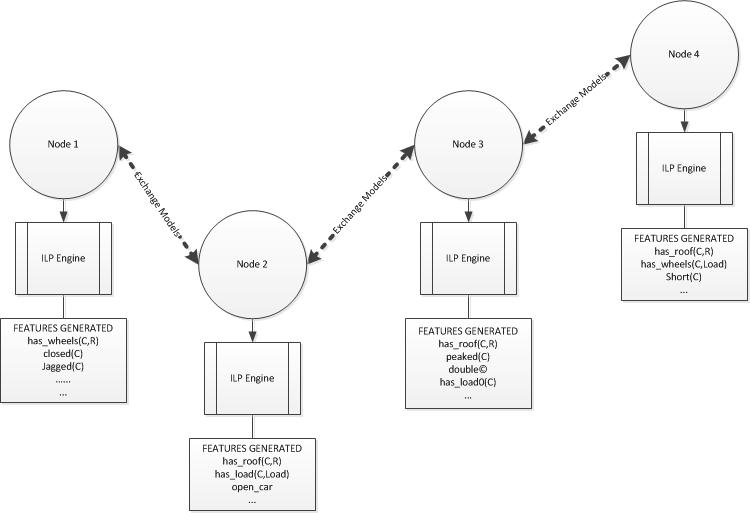
\includegraphics[height=0.50\textheight]{ilp_dfe.jpg}}
\caption{An illustrative example of the consensus-based approach using Michalski's ``Trains" problem \protect{\cite{Larson_77}}.
Each node has local features generated from an ILP engine, builds local models, estimates loss and shares
information with its neighbors. Eventually we would like all nodes to converge to the same model.}
\label{illEx}
\end{figure}





%The rest of the paper is organized as follows. Section \ref{sec:example}
%shows an example of what we expect to achieve, using a simple synthetic
%problem;
\noindent \textbf{Organization: } 
%Section \ref{sec:ilp} is a short introduction to ILP and its use in constructing features. 
Section \ref{conModel} formulates the problem as one of consensus-based model construction. Section \ref{sec:alg}
presents an iterative procedure for constructing models in a network of nodes capable
of exchanging information about their local models. Experimental
results are in Section \ref{sec:expt}. Section \ref{sec:related} presents related work; Section \ref{sec:concl} discusses open
issues and concludes the paper.

%\section{Distributed Feature Construction with ILP}
%\label{sec:example}
%
%We motivate the task of distributed feature construction using
%the train spotting problem, originally proposed by Ryzhard Michalski \cite{Larson_77}.
%Given two sets of trains: eastbound and westbound, the problem is to determine
%decision rules to distinguish between train sets, using properties of the
%carriages and load carried.
%% (Figure~\ref{trains}).
%%
%%\begin{figure}[htb]
%%\centerline{\includegraphics[width=1\textwidth,height=0.32\textheight ]{trains.jpg}}
%%\caption{The train spotting dataset. There are two sets of trains: Eastbound and Westbound. Descriptors for the trains include: number, shape and lengths of the car, shape of load, and so on. The task is to determine decision rules to distinguish between them. }
%%\label{trains}
%%\end{figure} 
%%
%%\noindent
%In \cite{michie:eastwest},
%a number of different theories are described for this data:
%
%\begin{description}
%\item[Theory A.] If a train has a short closed car, then it is Eastbound and
%    otherwise Westbound;
%\item[Theory B.] If a train has two cars, or has a car with a jagged roof, then it
%    is Westbound and otherwise Eastbound;
%\item[Theory C.] If a train has more than two different kinds of load, then it is
%    Eastbound and otherwise Westbound; and even, incredibly,
%\item[Theory D.] For each train add up the total number of sides of loads (taking
%    a circle to have one side). If the answer is a divisor of 60 then the train
%    is Westbound and otherwise Eastbound.
%\end{description}
%
%\noindent
%The reader will easilly be able to reformulate these rules as statements in
%propositional logic, using a language that contains symbols that are true if:
%a train has a short, closed car; a train has two cars; a train has a car with a jagged
%roof; a train is carrying dis-similar loads and so on. Further reflection may suggest
%that in fact, these propositions simply Boolean functions that, when given a
%structured description of a train, compute a value that is true or false.
%%For
%%example, the first proposition using the predicates (relations)
%%$HasCar$, $Short$ and $Closed$ is:
%%
%%\[
%%{f_1}(x)  = \left\{
%%\begin{array}{ll}
%%1 & \exists(HasCar(x,y) \wedge Short(y) \wedge Closed(y)) \\
%%0 & \mbox{otherwise}
%%\end{array}
%%\right.
%%\]
%%
%%\noindent
%Assuming that objects and situations can be adequately described by
%predicates, one very useful role for an ILP engine has been the discovery
%of ``good'' feature-functions, given data described in
%predicate-form
%(see, for example: \cite{Specia_09}). The approach used is similar to
%those adopted in data mining, with the ILP engine constructing a number
%of ``interesting features'' based on usual measures like support and recall.
%
%In data analysis, the ability to construct new features from primitive descriptions
%is clearly important. However, as can be seen from Theories A--D above, there may be very many possible features.
%Finding interesting elements in the space of all possible relational features requires data and
%involves a computationally intensive search process.
%It is, of course possible to contemplate the following
%approach: once the data are available, construct all, or a large number, of
%interesting features using an ILP engine; and then use some established methods of heuristic
%feature-selection when constructing models using these features. Assuming two
%substantial computational burdens can be overcome (large-scale feature
%construction, and large-scale feature selection), this approach would probably yield
%reasonable results. 
%



\section{Consensus-Based Model Construction}
\label{conModel}

\subsection{Problem Description}
\label{sec:probdesc}
Let $M$ denote an $n \times m$ matrix with real-valued entries.  This matrix 
represents a dataset of $n$ tuples of the form $X_i \in \mathbb{R}^m, 1 \le i \le n$.    
Assume, without loss of generality, this dataset has been vertically distributed over
$k$ sites $S_1, S_2, \cdots, S_k$ i.e. site $S_1$ has $m_1 $ features, $S_2$ has $m_2$ features
and so on, such that $|m_1| + |m_2|+ \cdots + |m_k| = |m|$,
where $|m_i|$ represents the number of features at site $S_i$\footnote{In the more general setting,
Site $S_i$ has a random subset of features $m_i \subset m$.}. 
Let $M_1$ denote the $n \times m_1$ matrix representing the dataset held by $S_1$,
$M_2$ denote the $n \times m_2$ matrix representing the dataset held by $S_2$ and so on.
Thus, $M = M_1:M_2: \cdots : M_k$ denotes the concatenation of the local datasets. 

We want to learn a linear discriminative function over the data set $M$. The global function to be
estimated is represented by $f_{g} = M W_{g}^{T} $ where $W_g$ is assumed to be a $1 \times m$ weight vector.
If only the local data is used, at site $S_1$, the local function estimated would be $f_1 = M_1 W_{1}^{T}$.
At site $S_2$, the local function estimated would be $f_2 = M_2 W_{2}^{T}$.
The goal is to describe a de-centralized algorithm for computing the weight vectors at sites $S_1, \cdots S_k$
such that on termination $W_{1} \approx W_g[1:m_1], W_2 \approx W_g[1:m_2], \cdots W_k \approx W_g[1:m_k]$
where $W_g[1:m_i]$ represents the part of the global weight vector for the attributes stored at that site $S_i$.
Clearly, if all the datasets are transferred to a central location, the global weight vector can be estimated.
Our objective is to learn the function in the decentralized setting assuming that transfer of actual data tuples is
expensive and may not be allowed (say for example due to privacy concerns). The weights obtained at each site on
termination of the algorithm will be used for ranking the features.

\begin{algorithm}[t]
\small
{
\SetKwData{Left}{left}\SetKwData{This}{this}\SetKwData{Up}{up}
\SetKwFunction{Union}{Union}\SetKwFunction{FindCompress}{FindCompress}
\SetKwInOut{Input}{input}\SetKwInOut{Output}{output}

%\Input{$n \times m_i$ matrix at each site $S_i$; \\
%      $G(V, E)$ which encapsulates the underlying communication framework; \\
%      $T: $ no of iterations} 
\KwIn{$n \times m_i$ matrix at each site $S_i$, $G(V, E)$ which encapsulates the underlying communication framework, $T: $ no of iterations }
\KwOut{Each site $S_i$ has $W_i \approx W_g[1: m_i]$ }
%\Output{Each site $S_i$ has $W_i \approx W_g[1: m_i]$ }
\BlankLine

 %
 %\KwData{$n \times m_i$ matrix at each site $S_i$; Graph $G(V, E)$ which encapsulates the underlying communication framework; $T: $ no of iterations}
 %\KwResult{Each site $S_i$ has $W_i \approx W_g[1: m_i]$ }
 %initialization\;
\For{t = 1 to T}
 {
  (a) Site $S_i$ computes $M_i W_i^T$ locally and estimates the loss function\;
  (b) Site $S_i$ gossips with its neighbors $S_j \in \{N_i\}$ and obtains $M_j W_j^T$ for each neighbor\;
  (c) Site $S_i$ locally updates its function estimate as $J_i^t = \alpha_{ii}(M_i W_i^T) + \alpha_{ji} (M_j W_j^T)$ \;
  (d) Update the local weight vectors using stochastic gradient descent as follows:
        $\frac{\partial L_p}{\partial W_i} = -X_p (Y_p - J_i^t(W_i^t(p)))$\;
  (e) If there is no significant change in the local weight vectors of one of the sites then stop
 }
 
\caption{Distributed Feature Estimation (DFE) by Consensus-Based Modeling}
\label{alg:fs}
}
\end{algorithm}

\subsection{Algorithm}
\label{sec:alg}

 We state the following assumptions under which the distributed algorithm operates:
%\subsubsection{Assumptions: }
%\label{assum}

\begin{asm}{Model of Distributed Computation.}
The distributed algorithm evolves over discrete time with
respect to a ``global'' clock\footnote{Existence of this clock is of interest only for theoretical analysis.}.
Each site has access to a local clock. Furthermore, each site has its own memory and can perform local
computation (such as computing the gradient on its local attributes). It stores $f_i$, which is the estimated local
function. Besides its own computation, sites may receive messages from their neighbors which will help in
evaluation of the next estimate for the local function.
\end{asm}

\begin{asm}{Communication Protocols.}
Sites $S_i$ are connected to one another via an underlying communication framework
represented by a graph $G (V, E)$, such that each site
$S_i \in \{S_1, S_2, \cdots , S_k\}$ is a vertex and an edge $e_{ij} \in E$ connects sites $S_i$ and $S_j$.
Communication delays on the edges in the graph are assumed to be zero.
It must be noted that the communication framework is usually expected to be application dependent.
In cases where no intuitive framework exists, it may be possible to simply rely on the physical connectivity of the machines,
for example, if the sites $S_i$ are part of a large cluster.
\end{asm}


Algorithm~\ref{alg:fs} describes how the weights for attributes will be estimated using a
consensus-based protocol. There are two main sub-parts of the algorithm:
(1) Exchange of local function estimate and (2) Local update based on stochastic gradient descent. Each of these sub-parts are discussed in further detail below.   Furthermore, assume that $J: R^m \rightarrow [0, \infty]$ is a continuously differentiable nonnegative cost function with a Lipschitz continuous derivative.\\

\noindent \textbf{Exchange of Local Function Estimate:}  Each site locally computes the loss based on its attributes and then gossips with the neighbors to get information on other attributes.
On receiving an update from a neighbor, the site re-evaluates $J_i$ by forming a component-wise convex combination of its old vector and the values in the messages received from neighbors i.e.   
 $J_i^{t+1}=\alpha_{ii}(X_i W_i^T) + \alpha_{ji} (X_j W_j^T)$. 
It is interesting to note that $\alpha_{ij}, 0 \le \alpha_{ij} \le 1$, is a non-negative weight that captures the fraction of information site $i$ is willing to share with site $j$. The choice of $\alpha_{ij}$ may be deterministic or randomized and may or may not depend on the time $t$ \cite{Kempe_03}. The $k\times k$ matrix $A$ comprising of $\alpha_{ij}, 1 \le i \le k, 1 \le j \le k$ is a ``stochastic" matrix such that it has non-negative entries and each row sums to one. More generally, this reflects the state transition probabilities between sites. Figure~\ref{stateTrans} illustrates the state transition between two sites $S_i$ and $S_j$. 

Another interpretation of the diffusion of $J_i$ amongst the neighbors of $i$ involves drawing analogies from Markov chains -- the diffusion is mathematically identical to the evolution of state occupation probabilities. Furthermore, a simple vector equation can be written for updating $J_i^t$ to $J_i^{t+1}$ i.e. $J_i^{t+1} = A(i) (J_i^t)_{N_i}$ where $A(i)$ corresponds to the row $i$ of the matrix $A$ and $(J_i^t)_{N_i}$ is a matrix that has $|N_i|$ rows (each row corresponding to a neighbor of Site $S_i$) and $n$ columns (each column corresponding to all the instances). More generally, $\mathcal{J}^{t+1} = A \mathcal{J}^{t}$ where $\mathcal{J}^{t+1}$ is a $k \times n$ matrix storing the local function estimates of each of the $n$ instances at site $k$ and $A$ is the $k \times k$ transition probability matrix corresponding to all the sites. It follows that $lim_{t \rightarrow \infty} A^t$ exists and this controls the rate of convergence of the algorithm. 

\begin{figure}[t]
\centerline{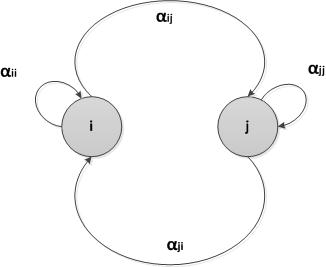
\includegraphics[height=0.28\textheight]{stateTrans.jpg}}
\caption{State Transition Probability between two sites $S_i$ and $S_j$}
\label{stateTrans}
\end{figure}

We introduce the notion of \emph{average function estimate} in the network $\vec{J_i^t} = \sum_i \frac{J_i^t}{k}$ which allocates equal weight to all the local function estimates and serves as a baseline against which individual sites $S_i$'s can compare their performance. Philosophically, this also implies that each local site should at least try to attain as much information as required to converge to the average function estimate. Since $\sum_i{\alpha_{ij}}=1$, this estimate is invariant. 

The $A$ matrix has interesting properties which allow us to show that convergence to $\vec{J_i^t}$ occurs. One such property is the Perron-Frobenius theory of irreducible non-negative matrices. We state the theorem here for continuity.

\begin{thm} \textbf{Perron-Frobenius \cite{Varga_62}}
Let $A$ be a positive, irreducible matrix such that the rows sum to 1. Then the following are true:
\begin{enumerate}
\item The eigenvalues of $A$ of unit magnitude are the $k$-th roots of unity for some $k$ and are all simple.
\item The eigenvalues of $A$ of unit magnitude are the $k$-th roots of unity if and only if $A$ is similar under a permutation to a $k$ cyclic matrix
\item all eigenvalues of $A$ are bounded by 1.
\end{enumerate}
\end{thm}

Since the eigenvalues of $A$ are bounded by 1, it can be shown that $J_i^t$ converges to the average function estimate $\vec{J_i^t}$ if and only if -1 is not an eigen value \cite{Varga_62}. 
Let $\lambda_n \le \lambda_{n-1} \le \cdots \le \lambda_2 < \lambda_1 =1$ be the eigenvalues of $A$ with $\lambda_1 = 1$. Also assume that $\gamma (A) = \text{max}_{i>1} |\lambda_i|$. It can be shown that $\parallel J_i^{t+1} - \vec{J}_i^{t} \parallel^2 \le \gamma^2 \parallel J_i^{t} - \vec{J}_i^{t} \parallel$. If $\gamma=1$, then system fails to converge \cite{Varga_62}, \cite{Cybenko_89}. \\
 
 
\noindent \textbf{Local Stochastic Gradient update} is done as follows: $W_i^{t+1} = W_i^t - \eta_i^t s_i^t$ where $s_i^t=\frac{\partial J_i^t}{\partial W_i^t} (X_r, W_i^t), X_r \in \mathbb{R}^{m_i}$ is the estimated gradient, $W_i^t$ is the weight vector and $\eta_i^t$ is the learning rate at node $i$ at time t. 




%For reasons of space, we omit the proof concerning the convergence of this algorithm (and
%the assumptions under which this proof holds).
%The proof of convergence of the algorithm has several sub-parts:
%(1) In the distributed setting, the process of information exchange between $k$ sites can be modeled as a
%non-stationary Markov chain. A non-stationary Markov chain is weakly ergodic if the dependence on the state distribution
%vanishes as time tends to infinity. Thus convergence of information exchange between sites needs to be established.
%This follows from the idea introduced by Tsitsiklis et al. \cite{Tsitsiklis_86}. It is based on proving convergence of a
%sequence of products of stochastic matrices (the $A$ matrix in our formulation) and the conclusions follow from
%well-known results on weak ergodicity of non-stationary Markov chains.
%(2) In a given iteration of the optimization, one needs to establish how good the approximated distributed optimization
%is compared to its ``ideal" central counterpart. This follows from the rich theory of approximate convex functions.
%We refer the reader to \cite{haimonti:dfetrep} for details.
%Here we focus
%on investigating the empirical behaviour of the consensus-based algorithm.
%
%Each of these sub-parts are discussed in further detail below.
%Furthermore, assume that $J: R^m \rightarrow [0, \infty]$ is a continuously differentiable
%nonnegative cost function with a Lipschitz continuous derivative.
%

\subsection{Convergence}
\label{sec:algterm}
%[READ CAREFULLY AND GIVE REFERENCE TO APPENDIX]
The proof of convergence of the algorithm makes use of the following concept: In the distributed setting, the process of information exchange between $k$ sites can be modeled as a non-stationary Markov chain. A non-stationary Markov chain is weakly ergodic if the dependence on the state distribution vanishes as time tends to infinity \cite{Tsitsiklis_86}. A detailed discussion regarding convergence of the algorithm is presented here. \\

%(2) The optimization of the cost function makes use of a stochastic gradient descent based technique.
%Thus convergence of information exchange between sites needs to be established. This follows from the idea introduced by Tsitsiklis et al. \cite{Tsitsiklis_86}. It is based on proving convergence of a sequence of products of stochastic matrices (the $A$ matrix in our formulation) and the conclusions follow from well-known results on weak ergodicity of non-stationary Markov chains. (2) In a given iteration of the optimization, one needs to establish how good the approximated distributed optimization is compared to its ``ideal" central counterpart. 
%\subsubsection{Analysis}

\noindent First, we make the following assumptions about the cost function $J$.
\begin{asm}{}
\begin{itemize}
\item $J(W^t) \ge 0$, for every $W^t \in R^m$.

\item \textbf{Lipschitz Continuity of $\nabla J$: } The function $J$ is continuously differentiable and there exists a constant $K_1$ such that 
\begin{equation}
\parallel \nabla J(W^{t_1}) - \nabla J(W^{t_2}) \parallel \le K_1 \parallel W^{t_1} - W^{t_2} \parallel, \forall \text{ } W^{t_1}, W^{t_2} \in \mathbb{R}^m.
\end{equation}

\item \textbf{Descent Lemma \cite{Bertsekas_97} } If $J$ satisfies the Lipschitz condition above, then
\begin{align*}
\label{desLips}
J(W^{t_1}+W^{t_2}) &\le J(W^{t_1}) + (W^{t_2})^{'} \nabla J(W^{t_1}) + \frac{K_1}{2} \parallel W^{t_2}\parallel_2^2,  \\
                    &\text{for all }W^{t_1}, W^{t_2} \in \mathbb{R}^m.
\end{align*}
\end{itemize}
\end{asm}
\noindent Proof of the above Lemma is presented in the Appendix and is along the lines of the argument presented in \cite{Bertsekas_97}.


\noindent In our algorithm, the vector $W^t$ is split over sites $S_1, S_2, \cdots, S_k$. The attributes at site $S_i, (1 \le i \le k) $ are updated according to the following equation:
\begin{equation}
W_i^{t+1} = W_i^t - \eta_i^t s_i^t
\end{equation} 
where $\eta_i^t$ is the step size and $s_i^t$ is the descent direction at site $S_i$. Let $T^i$ be the set of times when processor $i$ makes an update. It is assumed that $s_i^t=0$ when $t \notin T^i$. For times $t \in T^i$, we assume that the update direction is such that the cost function decreases and $s_i^t$ has the opposite sign from $\nabla J_i(W_i^{t})$. The underlying deterministic gossip algorithm is described by:
%let $\tau^{t}_{i}$ denote the time at which message $W_j^t$ (received by $i$ at time $t$) was transmitted by processor $j$. The message received by processor $i$ at time $t$ is equal to $W_j^t (\tau^{t}_{ij})$.  
%we have 
\begin{equation}
\label{gossip}
W_{i}^{t+1} = \sum_{\{i|t \in T^{i} \}} \alpha_{ii} W_{i}^{t} + \sum_{\{j|t \in T^{i} \}} \alpha_{ij} W_{j}^{t} \end{equation}
\noindent where the coefficients $\alpha$'s  are non-negative scalars.

\begin{ex}
Let $S_i$ and $S_j$ be the only two sites communicating with each other. Then equation~\ref{gossip} reduces to 
\begin{align*}
W_{i}^{t+1} &= \alpha_{ii} W_{i}^{t} + \alpha_{ij} W_{j}^{t} \\
            &= \alpha_{ii} (W_{i}^{t-1} - \eta_i^{t-1} s_i^{t-1}) + \alpha_{ij} (W_{j}^{t-1} - \eta_j^{t-1} s_j^{t-1}) \\
            &= (\alpha_{ii} W_{i}^{t-1} + \alpha_{ij}W_{j}^{t-1}) - ( \alpha_{ii} \eta_i^{t-1} s_i^{t-1} + \alpha_{ij}\eta_j^{t-1} s_j^{t-1}) \\
            &= \cdots \\            
            &= (\alpha_{ii} W_{i}^{1} + \alpha_{ij}W_{j}^{1}) - (\alpha_{ii} (\eta_i^{t-1} s_i^{t-1}+\eta_i^{t-2} s_i^{t-2} \cdots +\eta_i^{1} s_i^{1} ) \\
             &+ \alpha_{ij} (\eta_j^{t-1} s_j^{t-1} + \eta_j^{t-2} s_j^{t-2} + \cdots + \eta_j^{1} s_j^{1}) )    
\end{align*} 
\end{ex}

Hence, by induction it can be shown that:
\begin{equation}
\label{gos1}
W_{i}^{t} = \sum_{j=1}^{k} \alpha_{ij}W_{j}^{1} + \sum_{\tau=1}^{t-1}\sum_{j=1}^{k} \alpha_{ij}\eta_j^{\tau} s_j^{\tau}
\end{equation}
%The above can be proved by induction, using the fact that the composition of two linear functions is linear \cite{Bertsekas_89}. 
It is also assumed that there exist positive constants $K_4$ and $K_5$ such that step-sizes $\eta_i^{t}$ are bounded as follows:
$\frac{K_4}{t} \le \eta_i^{t} \le \frac{K_5}{t}$. Furthermore, the following assumptions hold true:

\begin{asm}
\begin{enumerate}
\item $\forall i, j$ and $0 \le \tau \le t$, $0 \le \alpha_{ij} \le 1$.
\item For any $i, j$ and $\tau \ge 0$, the limit of $\alpha_{ij}$ as $t$ tends to infinity exists and is the same for all $i$ and is denoted by $\alpha_{i}$
\item There exists some $\eta > 0$ such that $\alpha_{j} \ge \eta $ and $\forall j \in \{1, \cdots, k\}$ and $\tau \ge 0$
\item There exists constants $A > 0$ and $\rho \in (0,1) $ such that $|\alpha_{ij} - \alpha_{j}| \le A \rho^{t-\tau}, \forall t> \tau >0$
\end{enumerate}
\end{asm}

\begin{asm}
\label{asm1}

\noindent \textbf{Extensions of the Descent Lemma \cite{Bertsekas_97} at each site:} \\ 
(a) For every $i$ and $t$ we have,
\begin{equation}
s_i^t \nabla J_i(W_i^{t}) \le 0.
\end{equation}

\noindent (b) There exist positive constants $K_2$ and $K_3$ such that
\begin{equation}
K_2 |\nabla J_i(W_i^{t})| \le |s_i^t| \le K_3 |\nabla J_i(W_i^{t})|
\end{equation}
\end{asm}

%\noindent The lower bound on $|s_i^t|$ is introduced because otherwise $s_i^t$ could always be zero and in this case convergence cannot be demonstrated. The upper bound prevents the algorithm from exhibiting unstable oscillations.\\


\noindent Let $\mathcal{S}(t)$ be the set of random variables defined by: 
$\mathcal{S}(t)=\{s_i^{\tau}| i \in \{1, \cdots,k \}, \tau < t \}$. The variables in $\mathcal{S}(t)$ are the only sources of randomness upto the time $t$ at site $i$. The set $\mathcal{S}(t)$ is also a representation of the entire history of the algorithm upto the moment that the update directions $s_i^{\tau}$ are generated.

\begin{asm}
\label{as2}

\noindent \textbf{Stochastic Descent Lemma \cite{Bertsekas_97} at each site:} \\
There exist positive constants $K_6$, $K_7$ and $K_8$ such that: \\
(a) \begin{equation}
\label{descent01}
\nabla J(W_i^{t})' E[s_i^t|\mathcal{S}(t)] \le - K_6 \parallel \nabla J(W_i^{t}) \parallel^2, \forall t \in T^i.
\end{equation} \\
(b)\begin{equation}
\label{descent02}
 E[\parallel s_i^t \parallel^2|\mathcal{S}(t)] \le K_7 \parallel \nabla J(W_i^{t}) \parallel^2 + K_8,  \forall t \in T^i.
\end{equation} 
\end{asm}
\noindent \ref{asm1} implies that the expected direction of the update given the past history is in the descent direction. In \ref{as2} the presence of constant $K_8$ in the inequality allows the algorithm to make non-zero updates even when the minimum has been reached. \\

\begin{asm}

\noindent \textbf{Partial Asynchronism \cite{Bertsekas_97})} \\
There exists a positive integer $B$ such that: \\
(a) For every $i$ and for every $t \ge 0$ at least one of the elements of the set $\{t,t+1,\cdots,t+B-1\}$ belongs to $T^i$. \\
(b) There holds $\text{max}\{0,t-B+1\} \le \tau_{ij}^t \le t$, for all $i$ and $j$ and $t \ge 0$.
%If $J$ satisfies the Lipschitz condition of Assumption 1.0 (b) above, then:
%\begin{equation}
%J(W_i^t + W_j^t) \le J(W_i^t) + \frac{\partial J_j^{t}}{\partial W_j^{t}}\nabla J(W_i^t) + \frac{K}{2}||W_j^t||_2^2, \text{ for all } W_i^t, W_j^t \in R^m
%\end{equation}
\end{asm}
\noindent Finally, for completion we introduce the notions of \emph{martingales} and the martingale convergence theorem(s) which are required for the proofs in the appendix. 

A martingale is a model of a fair game where knowledge of past events never helps predict the mean of the future winnings. In general, a martingale is a stochastic process for which, at a particular time in the realized sequence, the expectation of the next value in the sequence is equal to the present observed value even given knowledge of all prior observed values at a current time\footnote{http://en.wikipedia.org/wiki/Martingale$\_$(probability$\_$theory)}. A formal definition (using measure theory \cite{Tao_11}) is given below:

Let $(\sigma, \mathcal{F}, P)$ be a probability space. A martingale sequence of length $n$, is a sequence $X_1, X_2, \cdots, X_n$ of random variables and corresponding sub-$\sigma$ fields $\mathcal{F}_1, \mathcal{F}_2, \cdots, \mathcal{F}_n$ that satisfy the following relations:
\begin{itemize}
\item Each $X_i$ is an integrable random variable which is measurable with respect to the corresponding $\sigma$-field $\mathcal{F}_i$.
\item The sigma fields are increasing $F_i \subset F_{i+1}$ for every $i$
\item For every  $i \in [1,2,\cdots,n-1]$, we have the relation, $X_i = E[X_{i+1}|\mathcal{F}_i]$ almost everywhere $P$. 
\end{itemize}

Along the same lines,
\begin{itemize}
\item A \emph{submartingale} is defined as: for every  $i$, $X_i \le E[X_{i+1}|\mathcal{F}_i]$ almost everywhere $P$ and 
\item A \emph{supermartingale} is defined as: for every  $i$, $X_i \ge E[X_{i+1}|\mathcal{F}_i]$ almost everywhere $P$. 
\end{itemize}

Martingale convergence theorem is a special type of theorem since the convergence follows from the structural properties of the sequence of random variables. The Supermartingale Convergence theorem and a variant used in proofs is presented next. \\

\noindent \textbf{Supermartingale Convergence Theorem \cite{Bertsekas_97}: } Let $\{Y_i\}$ be a sequence of random variables and let $\{\mathcal{F}_i\}$ be a sequence of finite sets of random variables such that $F_i \subset F_{i+1}$ for each $i$. Suppose that:
\begin{itemize}
\item Each $Y_i$ is non-negative
\item For each $i$, we have $E[Y_i] < \infty$
\item For each $i$, we have $E[Y_{i+1}|\mathcal{F}_i] \le Y_i$ with probability 1. 
\end{itemize}
Then there exists a non-negative random variable $Y$ such that the sequence of $\{Y_i\}$ converges to $Y$ with probability 1.\\

\noindent An extension of the above theorem, can be stated as follows:

Let $\{Y_i\}$ and $\{Z_i\}$ be two sequence of random variables. Let $\{\mathcal{F}_i\}$ be a sequence of finite sets of random variables such that $F_i \subset F_{i+1}$ for each $i$. Suppose that:
\begin{itemize}
\item The random variables $Y_i$ and $Z_i$ are non-negative.
\item There holds $E[Y_{i+1}|\mathcal{F}_i] \le Y_i+Z_i, \forall i$ with probability 1.
\item There holds $\sum_{i=1}^{\infty} E[Z_i] < \infty$.
\end{itemize}
Then there exists a nonnegative random variable $Y$ such that the sequence $\{Y_i\}$ converges to $Y$ with probability 1. \\



\noindent \textbf{Proposition 1.0. Convergence of the Distributed Feature Estimation (DFE) Algorithm } Under the Assumptions 1.0-3.0, there exists some $\eta^0 > 0$, such that if $0 < \eta_i^t < \eta^0$, then:
\begin{enumerate}
\item $\lim_{t \to \infty} J(W_i^t)$ exists and is the same for all $i$ with probability 1.
\item $\lim_{t \to \infty} (W_i^t - W_j^t)=0$ with probability 1 and in the mean square sense.
\item For every $i$, $\lim_{t \to \infty}\nabla J(W_i^t) = 0$.
\item Suppose that the set $\{W|J(W) \le C\}$ is bounded for every $C \in \mathcal{R}$; then there exists a unique vector $W^{*}$ at which $J$ is minimized and this is the unique vector at which $\nabla J$ vanishes. Then $W_i^t$ converges to $W^{*}$ for each $i$ with probability 1.
\end{enumerate}
 
 \noindent Proof in the Appendix.


\section{Empirical Evaluation}
\label{sec:expt}

\subsection{Aims}
\label{sec:exptaims}
Our objective is to investigate empirically the utility of the consensus-based
algorithm we have described. 
We use $Model(k,f)$ to denote the model returned by the consensus-based
algorithm in Section \ref{sec:alg}
using $k$ nodes in a network, each of which can call on an ILP engine to
construct at most $f$ features. In this section, we compare the
performance of: $Model(N,F)$ $(N > 1)$ with $Model(1,N \times F)$ The latter
effectively represents the model constructed in a non-distributed manner, with
all features present at a single centralised node. For simplicity, we
will call the former the $Distributed$ model and the latter the $Centralised$
model.

We intend to examine if there is empirical support for the conjecture
that the performance of the $Distributed$ model  is better than that of the $Centralised$ model.
We are assuming that the performance of a
model-construction method is given by the pair $(A,T)$
where $A$ is an unbiased estimate of the predictive accuracy of
the classifier, and $T$ is an unbiased estimate of the
time taken to construct a model. In all cases, 
the time taken to construct a model also includes the time taken to identify the
set of features by the ILP engine and the time to compute their values.
When $k > 1$, the time will also include
time for exchanging information. Comparison of
pairs $(A_1,T_1)$ and $(A_2,T_2)$ will simply be lexicographic comparisons. 


\subsection{Materials}
\label{sec:exptmat}


\subsubsection{Data}
Data for experiments are in two categories:
\begin{enumerate}
\item \textbf{Synthetic. } We use the ``Trains'' problem
    posed by R. Michalski for controlled experiments. Datasets
    of $1000$ examples
    are obtained for randomly drawn target concepts
    (see ``Methods'' below).\footnote{We note here that we are not concerned
    with large numbers of examples here, since the main investigation is
    concerned with subsets of the feature-space, and not of the data instances.}
    For this we use S.H. Muggleton's random train
    generator\footnote{{\tt http://www.doc.ic.ac.uk/$\mbox{}^\sim$shm/Software/GenerateTrains/}}                                                                                                                                             
    that defines a random process for generating examples. We will use this
    data for controlled experiments to test the principal conjecture
    about the comparative performances of $Distributed$ and $Centralised$ models.

\item \textbf{Real. } We report results from experiments conducted using $7$
    well-studied real world problems from the ILP literature. These are:
    Mutagenesis \cite{King_96}; Carcinogenesis \cite{King_96a}; DssTox \cite{Muggleton_08a};
    and 4 datasets arising from the comparison of Alzheimer's drugs
    denoted here as $Amine$, $Choline$, $Scop$ and $Toxic$ \cite{Srinivasan_1996y}.
    Our purpose in examining performance
    on the real-data is twofold. First, we intend to see if the use of
    linear models is too restrictive for real problems. Second, we would like to see
    if the results obtained on
    synthetic data are reflected on real-world problems. We note that for
    these problems predictive accuracy is the primary concern.
\end{enumerate}

\subsubsection{Algorithms and Machines}

The DFE algorithm has been implemented on a
Peer-to-Peer simulator, PeerSim \cite{peersim}. 
This software sets up the network by initializing the nodes and the protocols to be used by them.
The newscast protocol, an epidemic content distribution and topology management
protocol is used. Nodes can perform actions on local data as well as communicate with
each other by selecting a neighbour to communicate with
(using an underlying overlay network).
In each communication step, they mutually update their approximations of the
value to be calculated, based on their previous approximations.
The emergent topology from newscast protocol has a very low diameter and is
very close to a random graph (\cite{Jelasity_04},\cite{Jelasity_05}). %Two different network sizes are used for experiments -- 10 or 25. The nodes can have a low (2) or high (8 or 23) degree for each network configuration.


The ILP system used in all experiments is Aleph \cite{Srinivasan_99a}.
The latest version of this program (Aleph 6) is available from the second author.
The Prolog compiler used is Yap\footnote{\url{http://www.dcc.fc.up.pt/~vsc/Yap/}} (version 6.2.0). The programs are executed on
a dual Quad-Core AMD Opteron 2384 processors equipped with 2.7 GHz processors, 32 GB RAM,
and local storage of $4 \times 146$ GB 15K RPM Serial attached SCSI (SAS) hard disks. 


\subsection{Method}
\label{sec:exptmeth}

For the synthetic data, we distinguish between ``simple'' targets
(comprising disjuncts of 1-4 features) and ``complex'' targets (comprising disjuncts of 8--12 features).\footnote{This
distinction between {\em simple\/} and {\em complex\/} is based on results from cognitive psychology which suggest that people find it 
difficult to remember concepts with larger than 7 disjuncts.}
We call this dimension ``Target''. Our method for experiments is straightforward:

\begin{enumerate}
\item For each value of $Target$ \\
    %Repeat $k$\footnote{network size = $k$} times:
      \begin{enumerate}
        \item Randomly draw a target concept from $Target$ \label{meth:drawtarget}
        \item Classify each data instance as $+$ or $-$ using the target concept
        \item Randomly generate a network with $N$ nodes
        \item For each node in the network:
            \begin{enumerate}
                \item Set the number of iterations $T$ and initialize the
                    learning parameter $\eta_i$ for the
                    node. It is assumed that all nodes agree on the initial choice of
                    $T$ and $\eta_i = \eta$. 
               \item Execute the algorithm described in Section \ref{alg:fs} for $T$ iterations
                    and the ILP engine restricted to constructing $F$ features
               \item Record the predictive accuracy $A$ of the (local) model along with
                          the time $T$ taken to construct the model (this includes
                          the feature construction time, and the feature computation time).
                          The pair $(A,T)$ is the performance of the $Distributed$ model for the concept.
            \end{enumerate}
%        \item Compute average values for the predictive accuracy and the times
%                taken for model construction for
%                the $N$ nodes. Call this the performance of \textbf{Linear+ILP+DFE}
        \item Using a network with a single node:
            \begin{enumerate}
                \item Execute the
                    algorithm described in Section \ref{alg:fs} for $T$ iterations, learning
                    parameter $\eta$, 
                    and the ILP engine restricted to constructing $N \times F$ features
               \item Record the predictive accuracy $A'$ of the mode along with the time
                    taken to construct the model $T'$ (again, this includes the feature construction
                    time and feature computation time).
                    The pair $(A',T')$ is the performance of the $Centralised$ model for the concept.
            \end{enumerate}
      \end{enumerate}
      \item Compare the performances of the $Distributed$ and the Centralised models for the concepts.
\end{enumerate}

\noindent
The following additional details are relevant:

\begin{enumerate}
\item Two sources of sampling variation result with this method. First, variations are possible with
        the target drawn in Step \ref{meth:drawtarget}. Second, to ensure that
        both $Distributed$ and $Centralised$ approaches are constructing features from the same feature-space,
        we employ the
        facility within Aleph of drawing features from an explicitly defined feature space (this
        is specified using a large tabulation of features allowed by the language constraints).
        Although only ``good'' features are retained (see below),
        sampling variations can nevertheless result for both $Distributed$ and $Centralised$ models
        from the step of drawing features. In effect, we are performing a randomized search for
        good features within a pre-defined feature space. We report averages for $5$ repetitions
        of draws for the target, and $5$ repetitions of the randomized search for a given target.
\item A target is generated as follows. For simple targets, the number of
    features is chosen randomly from the range 1 to 4. For complex concepts,
    the number of features is randomly chosen from the range 8 to 12. Features are
    then randomly constructed using the ILP engine, and their disjunction constitute the
    target concept.
\item As noted previously, data instances for controlled experiments are drawn
    from the ``Trains" problem. The data generator uses S.H. Muggleton's random
    train generator. This implements a random process in which each data instance
    generated contains the complete description of a data object (nominally, a ``train'').
\item An initial set of parameters needs to be set for the ILP engine to describe ``good''
    features.
    These include $C$, the maximum number of literals in any acceptable clause constructed by the
    ILP system; Nodes, the maximum number of nodes explored in any single search conducted by
    the ILP system; Minacc, the minimum accuracy required of any acceptable clause; and Minpos, the
    minimum number of positive examples to be entailed by any acceptable clause.
    $C$ and Nodes are directly concerned with the search space explored
    by the ILP system. Minacc and Minpos
    are concerned with the quality of results returned (they are equivalent to ``precision" and ``support" used
    in the data mining literature). We set $C=4$, Nodes=5000, Minacc=0.75 and
    Minpos=2 for our experiments here. There is no principled reason for these choices, other
    than that they have been shown to work well in the literature.
\item The parameters for the PeerSim simulator include the size of the network,
    degree distribution of the nodes and the protocol to be executed at each node.
    We report here on experiments with a distributed network with $N=10$ nodes.
    Each of these nodes can construct up to $F = 500$ features (per class) and
    the centralised approach can construct up to $N \times F = 5000$ features (per class).
%    The nodes can have a low (max 2) or high (varied between 8 and 23)
%    degree for each network configuration.
\item The experiments here use the Hinge loss function. The results reported
    are for values of $T$ that the stochastic gradient descent method starts
    to diverge.
\item The learning rate $\eta_i$ remains a difficult parameter in any SGD-based method. There is no
    clear picture on how this should be set. We have adopted the following domain-driven approach.
    In general, lower values of the learning rate imply a longer search. We use three different learning
    rates corresponding to domains requiring high, moderate and low amounts of search (corresponding to
    complex, moderate or simple target concepts). The corresponding learning rates are
    $0.01$, $0.1$ and $1$. We reiterate that there is no prescribed method for deciding these values,
    and better results may be possible with other values.
   The maximum number of iterations $T$ is set to a high value ($1000$). The algorithm
   may terminate earlier, if there are no significant changes to its weight vector.
 \item Since the tasks considered here are binary classification tasks, the performance of the
    ILP system in all experiments will be taken to be the classification accuracy of the
    model produced by the system. By this we mean the usual measure computed from
    a $2 \times 2$ cross-tabulation of actual and predicted classes of instances.
    We would like the final performance measure to be as unbiased as possible by the
    experimental estimates obtained during optimization, and estimates are reported on a holdout set.
\item With results from multiple repetitions (as we have here), it is possible to perform
    a Wilcoxon signed-rank test for both differences and accuracy and differences in time.
    This allows a quantitative assessment of difference in
    performance between the Distributed and the Centralised models. However, results with
    $5$ repetitions are unreliable, and we
    prefer to report on a qualitative assessment, in terms of the average of
    accuracy and time taken. 
\end{enumerate} 

A data instance in each of the real datasets is a molecule, and contains the
complete description of the molecule. This includes: (a) bulk properties, like
molecular weight, logP values etc.; and (b) the atomic structure of the molecule, along
with the bonds between the atoms. For these datasets, clearly
there are no concepts to be drawn, and sampling variation results
solely from the feature-construction process. We therefore only report
on experimental results obtained from repeating the randomised search for
features. Again, estimates of predictive accuracy are obtained from a holdout set.
For mutagenesis and carcinogenesis, each of the 10 computational nodes in the distributed
network constructs up to  500 features, and the centralised approach constructs up to 5000 features (per class). For
DssTox, we found there were fewer high precision features than the other two datasets.
So the nodes in the distributed network constructs up to 50 features and the centralised node up to 
500 features (per class)

\subsection{Results}
\label{sec:results}

We present first the main results from the from the experiments on synthetic data (shown in Fig.\ref{fig:tab1}).
The primary observations in these experiments are as follows:
(1) On average, as concepts vary, the distributed algorithm appears to achieve higher accuracies
    than the centralised approach, although the differences may not be significant for a randomly
    chosen concept;
(2) On average, as concepts vary, the time taken for model construction by the distributed approach
    can be substantially lower\footnote{Although not apparent in the tabulation, the time is dominated
    by the time for constructing features. As a result, we note that the ratio of times for the
    centralised and distributed approaches need not be (linearly) proportional to the number of nodes
    in the network. For example, the search for a large subset of good features conducted by the
    a centralised approach may take much longer than the search for several small subsets conducted
    by the distributed approach.}; and
(3) The variation in both accuracies and time with the distributed approach due to both changes
    in the concept, or due to repetitions of feature-construction appear to be less than
    the centralised approach.
    

Taken together, these results suggest that good, stable models can be obtained from the distributed
approach fairly quickly, and that the approach might present an efficient alternative to
a centralised approach in which all features are constructed by a single computational unit.

% simple time stats
% Centr: FeatConstr + FeatureEval + ModelConstr
% s1: 86.05 + 0.0 + 0.02 =    86.07
% s2: 579.54 + 0.01 + 0.1 =   579.65
% s3: 361.48 + 0.03 + 0.23 =  361.74
% s4: 637.16 + 0.0 + 0.13 =   637.29 
% s5: 591.76 + 0.02 + 0.14 =  591.92
% Distr: FeatConstr + FeatureEval + ModelConstr
% s1: 25.7 + 0.01 + 0.2 = 25.81
% s2: 67.8 + 0.00 + 0.01 = 67.81
% s3: 60.7 + 0.00 + 0.05 = 60.75 
% s4: 65.7 + 0.00 + 0.04 = 65.74    
% s5: 51.8 + 0.00 + 0.04 = 51.84
    
% complex time stats
% Centr: FeatConstr + FeatureEval + ModelConstr
% s3: 414.5 + 0.06 + 0.2 = 414.76
% s5: 96.6 + 0.02 + 0.1 =   96.72
% s7: 253.9 + 0.03 + 0.2 = 254.13
% s8: 313.7 + 0.02 + 0.2 = 313.92   
% s9: 34.4 + 0.02 + 0.2 =   34.62
% Distr: FeatConstr + FeatureEval + ModelConstr
% s3: 51.7 + 0.02 + 0.1 = 51.82
% s5: 19.1 + 0.01 + 0.04 = 19.15
% s7: 55.0 + 0.02 + 0.02 = 55.04 
% s8: 49.7 + 0.01 + 0.02 = 49.73    
% s9: 32.4 + 0.02 + 0.03 = 32.45


% simple time stats
% Centr: FeatConstr [+ FeatureEval + ModelConstr]
% r1: 86.05 
% r2: 72.21
% r3: 190.1
% r4: 138.54
% r5: 51.7
% Distr: FeatConstr [+ FeatureEval + ModelConstr]
% r1: 25.81
% r2: 39.01
% r3: 55.82
% r4: 38.33
% r5: 38.86  
% complex time stats
% Centr: FeatConstr [+ FeatureEval + ModelConstr]
% r1: 414.5
% r2: 421.98
% r3: 413.80
% r4: 405.73 
% r5: 396.08
% Distr: FeatConstr [+ FeatureEval + ModelConstr]
% r1: 51.70
% r2: 56.65
% r3: 48.96
% r4: 51.91   
% r5: 55.04
\begin{figure}[htb]
% \begin{minipage}[h]{0.3\textwidth}
\begin{center}
{\small{
\begin{tabular}{|c|c|c||c|c|}\hline
Model & \multicolumn{2}{|c||}{$Simple$} & \multicolumn{2}{|c|}{$Complex$}\\ \hline
         & Acc.(\%)   & Time (s)        & Acc. (\%)  & Time (s) \\ \cline{2-5}
$Centr.$ & 83.3(14.4) & 0.12(0.07)& 92.0(7.1)  & 0.18(0.03) \\
$Distr.$ & 93.4(10.5) & 0.06(0.07)  & 98.7(1.2)  & 0.04(0.03)\\ \hline
\end{tabular}
}}
\end{center}
\begin{center}
(a) 
\end{center}
% \end{minipage}
% \begin{minipage}[h]{0.30\textwidth}
\begin{center}
{\small{
\begin{tabular}{|c|c|c||c|c|}\hline
Model & \multicolumn{2}{|c||}{$Simple$} & \multicolumn{2}{|c|}{$Complex$}\\ \hline
         & Acc.(\%)   & Time (s)       & Acc. (\%)  & Time (s) \\ \cline{2-5}
$Centr.$ & 83.6(20.1) & 0.14(0.07)& 95.3(0.6)  & 0.21(0.02) \\
$Distr.$ & 79.9(10.4) & 0.15(0.07)  & 96.6(0.6)  & 0.06(0.02)\\ \hline
\end{tabular}
}}
\end{center}
\begin{center}
(b)
\end{center}
% \end{minipage}

\caption{Results on synthetic data comparing $Centralised$ and $Distributed$ models.
        The results in (a) are averages from repetitions across concepts;
        and in (b) are averages from repetitions of the feature-construction process
        for a randomly drawn concept. In all cases, $Distributed$ denotes
        the model obtained with a $10$ node network, each of which employs
        a randomised search for up to 500 good features. $Centralised$ denotes
        the model obtained with a single node employing a randomised search
        for up to 5000 good features. All randomised searches draw features
        from the same feature-space.}
\label{fig:tab1}
\end{figure}%



What can we expect from the consensus-based learner on the real datasets? (Results are in Fig.\ref{fig:tab2}),
and we observe the following:
(1) There is a significant difference in accuracies between the distributed and
    centralised models on two of the datasets ($Canc330$ and $DssTox$). On balance,
    we cannot conclude from this that either one of the models is better;
(2) As with the synthetic data, the time for the distributed models is substantially lower.
    As before, the time is dominated by the feature-construction effort. For the real data sets,
    it appears that it is substantially easier to get smaller subsets of good features than larger ones
    (as observed from the substantial difference in the times between the distributed and centralised models); and
(3) Comparisons against the baseline suggest that the use of linear models is not overly restrictive, since the
    models obtained are not substantially worse (predictively speaking) than the ones obtained by ILP in the past.

Again, taken together, these results provide support to the trends observed with the controlled experiments and
suggest that the distributed approach would continue to perform at least as well as the centralised approach
on real data.


% Mut188
% Distr: Feature Gen [+ rest]

% 
\begin{figure}[htb]
\begin{center}
{\small{
\begin{tabular}{|c|c|c|c||c|c|c|}\hline
Problem & \multicolumn{3}{|c||}{$Acc$ (\%)} & \multicolumn{3}{|c|}{$Time$ (s)} \\ \hline
         & Centr.   & Distr. & Base. & Centr. & Distr. & Base. \\ \cline{2-7}
         
$Mut188$ & 84.3(2.6) &  76.8(0.0) & 84.6(2.6) & 1.93(0.53)& 0.42(0.02)    & --  \\
$Canc330$ & 67.6(0.5)& 56.8(0.5)  & 50.4(2.8) & 3.56(0.58) & 0.82(0.18) & -- \\
$DssTox$ & 53.8(0.0) &  61.6(1.0) & 64.7(2.0) & 1.94(0.91) & 0.76(0.48) & --\\
$Amine$  & 75.5(0.4) & 76.6(0.8) &  71.4(1.7)         &7.02(0.24) &0.87(0.11)           & -- \\
$Choline$& 72.9(1.3)  &71.2(0.7) &     52.7(1.4)      &13.00(3.06)  &1.64(0.5)           & -- \\
$Scop$   & 67.2(1.5)  & 69.9(0.3) &   55.1(2.0)        &11.9(0.64)&1.20(0.03)           & -- \\
$Toxic$  &  76.3(1.3) &81.4(0.2) &  79.2(1.4)         &7.44(3.51)&0.89(0.49)           & -- \\ \hline
\end{tabular}
}}
\end{center}
\caption{Results on real data comparing $Centralised$ and $Distributed$ models.
    The Baseline models are the ones reported in
    \protect{\cite{AshwinJMLR2012}} (these are cross-validation estimates, whereas the
    estimates for $Centralised$ and $Distributed$ models are from holdout sets). No
    estimates of time are reported in that paper.}
\label{fig:tab2}
\end{figure}


\noindent We turn now to some issues that have been brought out by the experiments:

\begin{figure*}[h]
\centering
{
	\subfigure[Variation in feature and model construction time for five repetitions of the feature-construction process for a randomly drawn simple target. ]
	{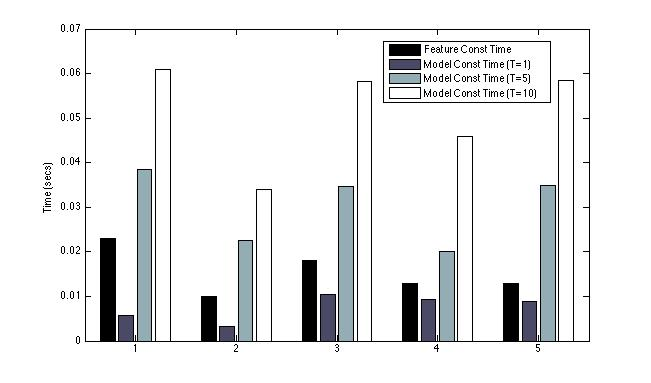
\includegraphics[width=0.85\textwidth, height=0.36\textheight]{simple-RepFeat.jpg}
	\label{simpleRepFeat}
	}
	\subfigure[Variation in feature and model construction time for five repetitions across concepts for simple targets.]
	{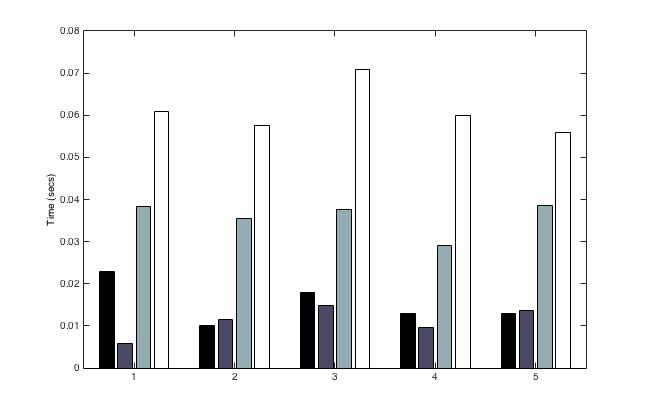
\includegraphics[width=0.85\textwidth,height=0.36\textheight]{simple-RepConcepts.jpg}
	\label{simpleRepConcepts}
	}
}
\caption{Simple Targets }
\end{figure*}

\begin{figure*}[h]
\centering
{
	\subfigure[Variation in feature and model construction time for five repetitions of feature-construction process for a randomly drawn complex target. ]
	{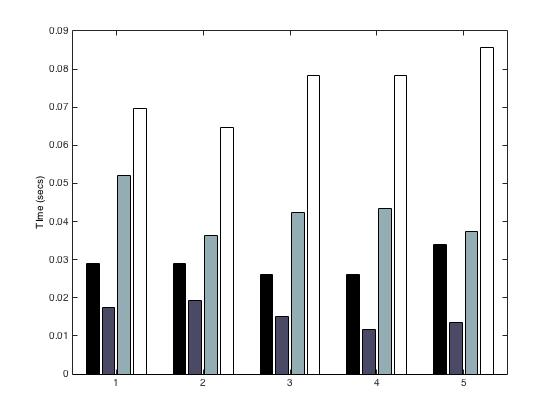
\includegraphics[width=0.8\textwidth, height=0.36\textheight]{complex-RepFeat.jpg}
	\label{comRepFeat}
	}
	\subfigure[Variation in feature and model construction time for five repetitions across concepts for complex targets.]
	{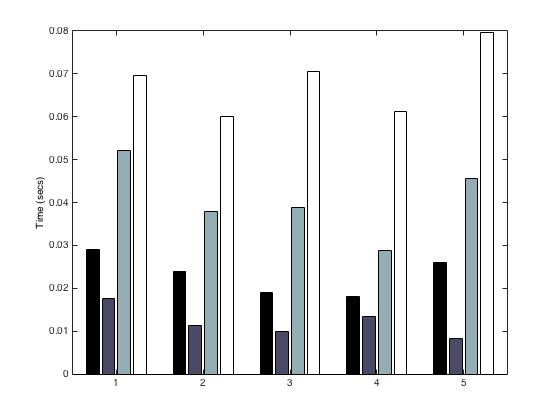
\includegraphics[width=0.75\textwidth,height=0.36\textheight]{complex-RepConcepts.jpg}
	\label{comRepConcepts}
	}
}
\caption{Complex Targets }
\end{figure*}

\begin{figure}[h]
\begin{minipage}[h]{0.5\textwidth}
\begin{center}
{\small{
\begin{tabular}{|c|c|c|}\hline
$\lambda$ & $Acc$ (\%) & $Time$ (s) \\ \hline

$0.01$ &92.4 &0.05  \\
$0.1$ & 92.4& 0.05\\
$1$ & 93.4& 0.06\\ \hline
\end{tabular}
}}
\end{center}
\begin{center}
(a) Simple
\end{center}
\end{minipage}
\begin{minipage}[h]{0.50\textwidth}
\begin{center}
{\small{
\begin{tabular}{|c|c|c|}\hline
$\lambda$ & $Acc$ (\%) & $Time$ (s) \\ \hline

$0.01$ & 98.7&  0.04\\
$0.1$ & 95.6& 0.05 \\
$1$ & 77.8& 0.37\\ \hline
\end{tabular}
}}
\end{center}
\begin{center}
(b) Complex
\end{center}
\end{minipage}

\caption{Effect of the learning rate $\lambda$.}
\label{fig:lambda}
\end{figure}

\begin{description}
    \item[The learning rate $\lambda$.] As with all methods based on stochastic gradient descent,
            the central parameter remains the learning rate $\lambda$. 
                Many strategies have been suggested in literature to automatically adjust the
            learning rates.
        (see for example
        \cite{bottou-2010}, \cite{bottou-bousquet-2011}, \cite{Darken_90}, \cite{Sutton_92}).
        In general, the learning rate on an iteration $\eta_i$ of the algorithm here is of the form $\eta_i = \frac{B}{T^{-\alpha}}$;
        $B=e^{-\lambda T}; 0 < \alpha \le 1$. Fig.~\ref{fig:lambda} shows the effect
        of varying $\lambda$ for the synthetic datasets used here.
        These results show that the
        determination of $\lambda$ is a tricky business, that can depend on the
        nature of the target theory being approximated (correctly, it
        is really to do with the amount of search needed).
        For experiments reported above, we have used fixed values
        of $\lambda$ based on our assessment of the search required
        (see the additional details in the Methods section).
        That $\lambda$ is dataset dependent and needs to
        assigned in some domain-dependent
        manner appears to be an unavoidable aspect of any SGD-based method.
  \item[Disaggregated Time.] The time estimates reported in the tabulations consist
        of four separate components. These are: (a) feature-construction;
        (b) feature-evaluation; (c) model-construction; and (d) inter-node communication.
        Components (a)--(c) are part of
        of both centralised and distributed learners, and it is of some interest
        to examine their separate contributions. %This is shown in Fig.~\ref{fig:time}(a)--(b).
        Feature evaluation is very small for both simple and complex trains ($<0.01\%$). Feature-construction is roughly $99\%$ of the time spent in feature engineering.
        
        We note that all experiments reported here use the PeerSim simulator,
        which does have provisions for modeling the transport layer
        via a special protocol that provides a message sending service.
        There are also options for modeling latency among geographically distributed nodes in
        addition to churn models for nodes. None of these aspects have been
        explored here, and the tabulation reported here use default
        settings of the simulator that are designed to model a network as a random graph.
        It is nevertheless evident that distributed
        model construction is only worthwhile provided communication costs are
        low---there will be real networks (and corresponding simulator settings)
        for which distributed model-construction can be a good or a
        bad approach.
        
        Figure~\ref{simpleRepFeat} and ~\ref{simpleRepConcepts} depicts the variation in the feature and model construction time for (a) repetitions of feature-construction process for a randomly drawn simple target and (b) repetition across simple concepts. For model construction, the number of iterations $T$ is varied between 1, 5 and 10. In all the cases, a single iteration of the stochastic gradient descent algorithm is good enough to obtain reasonably good accuracy in the distributed settings. Also, for small values of $T$, the feature construction time dominates communication costs. Similar figures for complex targets are presented in Figures~\ref{comRepFeat} and ~\ref{comRepConcepts}. 
        
%        \begin{figure}[t]
%	\centerline{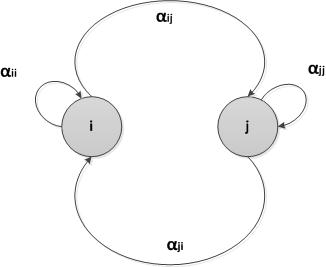
\includegraphics[height=0.28\textheight]{stateTrans.jpg}}
%	\caption{State Transition Probability between two sites $S_i$ and $S_j$}
%	\label{stateTrans}
%	\end{figure}
%
%\begin{figure}[t]
%\centerline{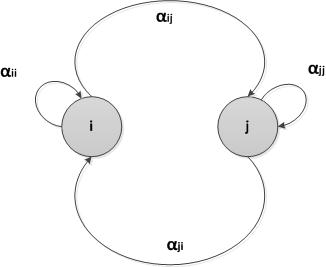
\includegraphics[height=0.28\textheight]{stateTrans.jpg}}
%\caption{State Transition Probability between two sites $S_i$ and $S_j$}
%\label{stateTrans}
%\end{figure}

        
        % (see Fig.~\ref{fig:time}(c)--(d)). 
 
 \begin{figure*}[h]
\centering
{
	\subfigure[ Repetition of the feature-construction process.]
	{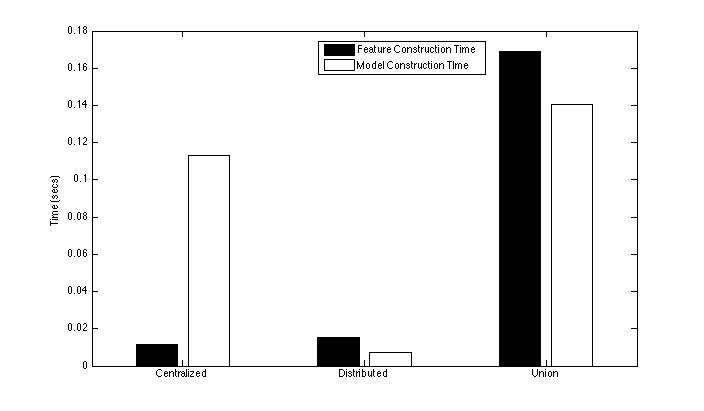
\includegraphics[width=0.85\textwidth, height=0.36\textheight]{simple-RepFeat-FeatMod.jpg}
	\label{simpleRepFeatMod}
	}
	\subfigure[Repetition across concepts.]
	{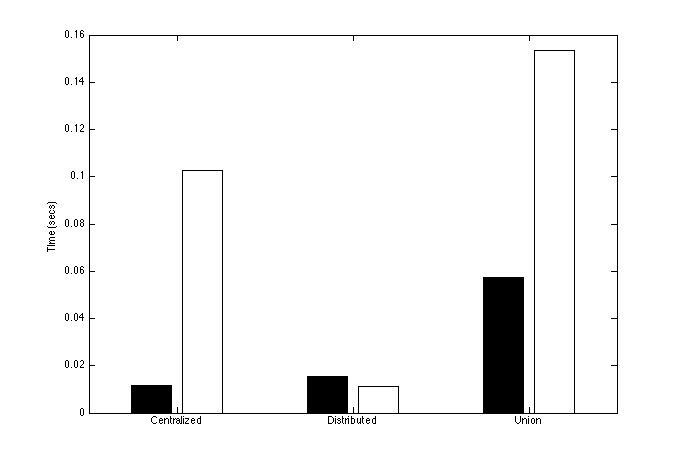
\includegraphics[width=0.85\textwidth,height=0.36\textheight]{simple-RepConcepts-FeatMod.jpg}
	\label{simpleRepConceptsFeatMod}
	}
}
\caption{Variation in feature and model construction time for a randomly drawn simple target. Three different strategies are compared -- Centralized, Distributed and Union.}
\label{fig:simpleUnion}
\end{figure*}

 \begin{figure*}[h]
\centering
{
	\subfigure[ Repetition of the feature-construction process.]
	{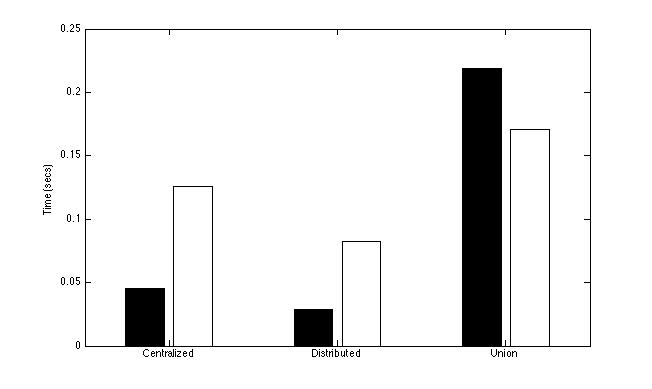
\includegraphics[width=0.85\textwidth, height=0.36\textheight]{complex-RepFeat-FeatMod.jpg}
	\label{complexRepFeatMod}
	}
	\subfigure[Repetition across concepts.]
	{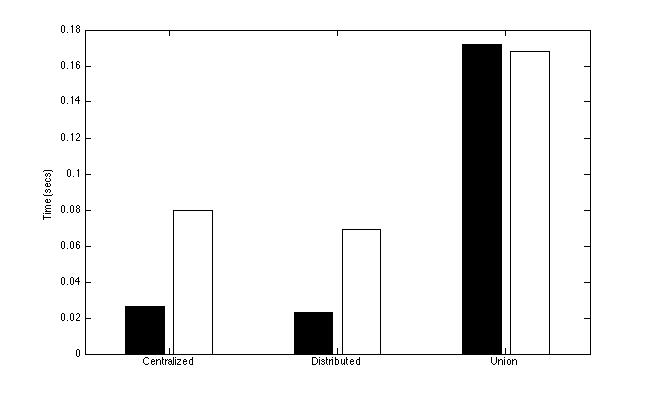
\includegraphics[width=0.85\textwidth,height=0.36\textheight]{complex-RepConcepts-FeatMod.jpg}
	\label{complexRepConceptsFeatMod}
	}
}
\caption{Variation in feature and model construction time for a randomly drawn complex target. Three different strategies are compared -- Centralized, Distributed and Union.}
\label{fig:complexUnion}
\end{figure*}

\begin{figure}[htb]
% \begin{minipage}[h]{0.3\textwidth}
\begin{center}
{\small{
\begin{tabular}{|c|c|c||c|c|}\hline
Model & \multicolumn{2}{|c||}{$Simple$} & \multicolumn{2}{|c|}{$Complex$}\\ \hline
         & Acc.(\%)   & Time (s)        & Acc. (\%)  & Time (s) \\ \cline{2-5}
$Feat.$ & 98.4(1.74) & 0.31(0.03)& 99.58(0.18)  & 0.39(0.02) \\
$Con.$ & 93.42(4.71) & 0.21(0.05)  & 95.66 (5.93)  & 0.34(0.04)\\ \hline
\end{tabular}
}}
\end{center}
\begin{center}
(a) 
\end{center}
% \end{minipage}

\caption{Results on synthetic data for ``Union" of features at a centralized node.
        The results corresponding to \emph{Feat.} are averages from repetitions of the feature-construction process
        for a randomly drawn concept while those for \emph{Con.} are averages from repetitions across concepts. In all cases, ``Union" denotes
        the model obtained by vertically concatenating data from all the nodes in network.}
\label{fig:tabUnion}
\end{figure}%
       
 \item [Union of Features.] A question that is imperative is, ``How good is the performance of the algorithm, if the centralized approach  were to use the exact union of all the features in the distributed setting?" The results presented in Table~\ref{fig:tabUnion} help answer this question. In general, the model(s) built on the ``Union" of features\footnote{Both the test and train data are concatenated vertically using data from all nodes in the network.} have comparable performance to the distributed algorithm presented here, but this comes at a price in terms of the computational effort required to build the models. Figures~\ref{fig:simpleUnion} and~\ref{fig:complexUnion} further analyze the time by dividing it into feature and model construction time(s). The cost of forming the ``Union" of features is significantly high in most cases compared to the model construction time.

    \item[Convergence Accuracy.] In experiments here (both with synthetic and real data), we have observed that
            the predictive accuracy of the model from the distributed setting is comparable to the predictive accuracy from
            the non-distributed setting. Unlike gains in time which can be expected from a distributed setting,
            it is not evident beforehand
            what can be expected on the accuracy front. This is because the models constructed in the two settings sample different
            sets of features. The results here suggest a conjecture that the consensus-based approach will always converge
            to model that is within some small error bound of the model from a centralized approach with the
            same number of features. We have some reason to believe that this conjecture may hold
            in some circumstances, based on the use of Sanov's theorem \cite{Sanov_57} and related techniques.
 \item[Network Topology.] Experiments have been designed to test the effect of the network topology on the convergence rate of the algorithm using synthetic data.  To simulate topologies using the PeerSim simulator, the following method is adapted: A tree is built as nodes arrive uniformly at random in a unit
square\footnote{The square shape is inconsequential.}, starting at the \emph{root} node denoted by $x_i$. When node $j$ arrives,
it attaches itself to an already existing node by minimizing the following formula: $W(x_j) + \alpha \text{dist}(x_i, x_j)$, where $\text{dist()}$ is the Euclidean distance and $\alpha$ is a weight parameter. Assuming $K$ to be the number of outgoing edges from a node, three different strategies of node addition are explored: (a) \textbf{Random: } $K$ nodes are added at random. (b)  \textbf{Star: } $K$ nodes are added in a star topology and (c) \textbf{Scale Free Network: } A scale-free network is grown using the Barabasi-Albert (BA) model ensuring that nodes have power law degree distributions. Two values of $K = 2, 8$ were used in empirical analysis. Our results indicate that there were no statistically significant difference in performance for the 10 node network(s) studied in this paper.


\end{description}


%\begin{figure}
%\begin{minipage}[h]{0.50\textwidth}
%\begin{center}
%{\small{
%\begin{tabular}{|l|c|c|}\hline
%$Time$ & $Simple$  & $Complex$ \\ \hline
%
%Feature Construction & &  \\
%Feature Evaluation  & & \\
%Model Construction  & & \\
%Communication       & & \\ \hline
%\end{tabular}
%}}
%\end{center}
%\begin{center}
%(a) Centralised
%\end{center}
%\vspace*{0.2cm}
%\end{minipage}
%\begin{minipage}[h]{0.50\textwidth}
%\begin{center}
%{\small{
%\begin{tabular}{|l|c|c|}\hline
%$Time$ & $Simple$  & $Complex$ \\ \hline
%
%Feature Construction & &  \\
%Feature Evaluation  & & \\
%Model Construction  & & \\
%Communication       & & \\ \hline
%\end{tabular}
%}}
%\end{center}
%\begin{center}
%(b) Distributed
%\end{center}
%\vspace*{0.2cm}
%\end{minipage}
%\begin{minipage}[h]{0.50\textwidth}
%\begin{center}
%{\small{
%\begin{tabular}{|l|c|c|}\hline
%$Time$ & $Simple$  & $Complex$ \\ \hline
%Feature Construction & &  \\
%Feature Evaluation  & & \\
%Model Construction  & & \\
%Communication       & & \\ \hline
%\end{tabular}
%}}
%\end{center}
%\begin{center}
%(c) Centralised
%\end{center}
%\end{minipage}
%\begin{minipage}[h]{0.50\textwidth}
%\begin{center}
%{\small{
%\begin{tabular}{|l|c|c|}\hline
%$Time$ & $Simple$  & $Complex$ \\ \hline
%Feature Construction & &  \\
%Feature Evaluation  & & \\
%Model Construction  & & \\
%Communication       & &  \\ \hline
%\end{tabular}
%}}
%\end{center}
%\begin{center}
%(d) Centralised
%\end{center}
%\end{minipage}
%\caption{Estimates of time spent in feature-engineering, model-construction and communication.
%(a)--(b) are for the network parameters used in the experiments here. }
%%(c)--(d)are for networks that have much lower or higher latencies respectively.}
%\label{fig:time}
%\end{figure}

\section{Related Work}
\label{sec:related}
%Feature selection improves learning performance, lowers computational complexity, and builds better generalizable models and these techniques have been studied extensively in literature. 
We review related work from several areas: large scale feature selection, decentralized
optimization and consensus-based learning, and discovery of feature subsets by ILP engines.

\noindent \textbf{Large Scale Feature Selection: }Techniques for selecting
from a (large) but finite set of features of known size $d$\footnote{A large feature set increases
the size of the search space, making it more difficult for the
learning algorithm to find a near optimal solution.}
have been well-studied within the machine learning community, usually under
the umbrella-terms of filter-based or wrapper-based methods
(see for example, \cite{John_94,Liu_98}). 
While most of the early work was intended for implementation on a single
machine, several algorithms have been proposed to enable feature-selection from massive datasets \cite{Garcia_06,Lopez_06,Sun_14}. Singh et al. \cite{SinghKLS09} propose a framework for handling feature selection for logistic regression by developing a new forward feature selection heuristic that ranks features by their estimated effect on the resulting model's performance. An approximate optimization, based on back fitting, provides a fast and accurate estimate of the coefficient for each new feature in the logistic regression model. Zhao et al. \cite{ZhaoCDS12} describe an algorithm that selects features based on their ability to explain data variance. Zhou et al. \cite{Zhou_14} present a framework for Parallelizable Feature Selection (PFS) which is inspired by the theory of group testing. Group testing is a combinatorial search paradigm where the goal is to identify a small subset of relevant items from a large pool of possible items. The feature selection problem in the group testing framework applies a ``test" to a set of features which produces
a score designed to measure the quality of the features. From the collection of test scores the relevant features are supposed to
be identified. The authors also make the claim that a sequential method is likely to take an unreasonably long time, thereby necessitating the development of a parallel algorithm.  PFS has several similarities to the algorithm proposed in this paper - notably, the set of features at each node can be viewed as a collection of \emph{relevant features} for group testing; the process of local function evaluation can be mapped to the ``test" required in group testing. The end product, however, in the two algorithms are fundamentally different - in PFS all feature sets are identified in advance without knowing the scores of other tests and a final subset of features is discovered; nodes executing the DFE algorithm have updated scores of the local features after gossiping with neighbors. The updated scores help learn approximations of the global objective and nodes independently reach a consensus.  

In the distributed setting, the data is partitioned and
placed on different processors; each processor learns a local objective from data stored on it; processors then communicate to find parameters that
minimize loss over the entire dataset. However, communication has to be fast
enough so that network latencies do not offset computational gains \cite{Kargupta_98a}. The data partitioning
scheme -- horizontal (all instances have the same features) or
vertical (instances have access to only a subset of features) plays an
important role in the design of distributed algorithms. Furthermore, distributed computation is utilized to solve optimization problems that arise when exploring huge, nonlinear and multidimensional search spaces. Distributed feature selection algorithms often solve decentralized optimization problems in the constrained and unconstrained settings (seminal work of Bertsekas, Tsitsiklis and colleagues \cite{Tsitsiklis_86,Tsitsiklis_84,Bertsekas_97}). The convergence properties of these decentralized optimization problems naturally affect the performance of the distributed feature selection algorithms. In recent work, it has been shown that convergence properties of distributed optimization algorithms of unconstrained optimization algorithms (such as gradient descent and its stochastic variants) can be related to the network topology of the underlying distributed infrastructure by using its spectral properties (\cite{Boyd_06,Shah_09,Dimakis_06,Benezit_10}).

%In addition, careful design of feature selection algorithms and communication protocols is required since it affects estimates of the global solution. Selection of a minimal subset of features locally according to some reasonable criteria, fundamentally involves finding a solution to one or more optimization problems. Local solutions must be communicated to neighbors enabling exchange of information. Distributed feature selection algorithms must therefore efficiently solve decentralized optimization problems. 

\noindent \textbf{Distributed Optimization: } Learning feature subsets in distributed environments using decentralized optimization
has become an active area of research(\cite{Duchi_12,Agarwal_14a,Chris_08}) in recent years. 
Agarwal et al. \cite{Agarwal_14a} present a system and a set of techniques for
learning linear predictors with convex losses on terabyte sized datasets.
Their goal is to learn problems of the form
$ \text{min }_{w \in R^d} \sum_{i=1}^{n} l (w^T x_i; y_i) + \lambda R(w)$
where $x_i$ is the feature vector of the $i^{th}$ example, $w$ is the weight vector
and $R$ is a regularizer. The data are split horizontally and examples are
partitioned on different nodes of a cluster. Duchi et al.
\cite{Duchi_12} present a dual averaging sub-gradient method which
maintains and forms weighted averages of sub-gradients in the network. An
interesting contribution of this work is the association of convergence of the
algorithm with the underlying spectral properties of the network.
Similar techniques for learning linear predictors have been presented
elsewhere (\cite{Mangasarian_95,McDonald_10,zinkevich_10},
\cite{Hogwild_11,Boyd_11}). The algorithm presented in this paper
differs from this body of literature in that the data are split
\emph{vertically} amongst nodes in the cluster thereby necessitating a
different algorithm design strategy. In addition, this is a batch algorithm and
hence quite different from distributed online learning
counterparts (\cite{Dekel_12a,Langford_09a,bottou_2011}).
Das et al. \cite{Das_10}
show that three popular feature selection criteria -- misclassification gain,
gini index and entropy can be learnt in a large peer-to-peer network.
This is then combined with protocols for asynchronous distributed
averaging and the secure sum protocols to present a privacy preserving
asynchronous feature selection algorithm.

%An unsupervised multi-view feature selection algorithm for object recognition or indexing from multiple cameras has been presented by Christoudias et al. \cite{Chris_08} where a Gaussian Process model of the joint view statistics is used at the receiver to obtain a joint encoding of views without directly sharing information across encoders. \\

%Aside from the fact that the emphasis of this algorithm is on privacy preservation, it must be noted that this algorithm works on horizontally partitioned data i.e. each peer has the same set of features but different tuples. In contrast, the algorithm presented here has been designed for vertically partitioned data.

\noindent \textbf{Discovery of feature subsets by ILP engines: }Existing literature on discovering a subset of interesting features from
large, complex search spaces such as those by ILP engines
adapt one of the following strategies:
\begin{enumerate}
 \item Optimally~\cite{l1Reg,cvpr2007,nips2004} or
    heuristically~\cite{JoshiRS08,Amrita12,Specia_09,RamakrishnanJBS07,SpeciaSRN06,NageshRCKDB12,ChalamallaNSR08}
    solve a discrete optimization problem.
 %Temporal ordering among features is studied by Nowizin et al.\cite{cvpr2007} while Han et al.\cite{l1Reg} introduce $l_1$ regularization into relational learning for sparse rule combination.
\item Optimally~\cite{JawanpuriaNR11,NairSRK12} solve a convex
    optimization problem with sparsity inducing regularizers; 
 \item Compute all relational features that satisfy some quality criterion by
    systematically and efficiently exploring a prescribed
    search space~\cite{pei2004,subseqGap2006,bitSpade,antunes2003,han2005,rakesh1995,han2004,gehrke2002,rastogi1999,davis2005integrated,Davis05b,Landwehr:2007,Davis:2007,Dzeroski:1993}.
\end{enumerate}

\noindent
Again, much of this has been of a non-distributed nature, and
usually assume a bound on the size of the feature-space. The latter
is not the case for a technique like the one proposed in
\cite{JoshiRS08}. This describes a randomized local search based
technique which repeatedly constructs features
and then performs a greedy local search starting from this
subset. Since enumeration of all local moves can be prohibitively large,
the selection of moves is guided by errors made by the model constructed
using the current set of features. Nothing is assumed about the size
of the feature-space, making it a form of vertical partitioning of the kind
we are interested in.
Multiple random searches can clearly be
conducted in parallel (although this is not done in the paper)~\cite{Filip_06a,Fonseca:2005}. As with
most randomized techniques of this kind, not much can be said about the
final model.
    
Perhaps of most interest to the work here is the Sparse
Network Of Winnow (SNoW) classifiers described in \cite{Roth_98,CCRR99}.
As it stands, this horizontally partitions the data into subsets, constructs
multiple linear models using Winnow's multiplicative update process, and
finally uses a majority vote to arrive at a consensus classification. This
would appear, on the surface to be quite different to what we propose here.
Nevertheless, there are reasons to believe that this approach can be usefully
extended to the setting we propose. It has been shown elsewhere that the
Winnow-based approach can be extended to an infinite-attribute setting \cite{Blum1992}. The
work in this paper shows that consensus linear models are possible when
convex cost functions are used. Finally, from the ILP-viewpoint, \cite{ashbain:stream} shows how
it is possible to construct Winnow-based models in an infinite-attribute
setting using an ILP engine with a stream-based model of the data. Taken together,
this suggests that a combination of the techniques we propose, and those in
\cite{CCRR99} can be used to develop linear models that can handle both
horizontal partitioning of the data and vertical partitioning of the feature-space.


\section{Conclusion}
\label{sec:concl}

A particularly effective form of Inductive Logic Programming has been its use
to construct new features that can be used to augment existing descriptors of
a dataset. Experimental studies reported in the literature have repeatedly shown
that the relational features constructed by an ILP engine can substantially assist
in the analysis of data. Models constructed in this way have looked at both classification
and regression, and improvements have resulted in each case. Practical difficulties
have remained to be addressed though. The rich language of first-order logic used
by ILP systems engenders a very large space of possible new features. The resulting
computational difficulties of finding interesting features is not
easily overcome by the usual ILP-based methods of language bias or constraints. In
this paper, we have introduced what appears to be the first attempt at the use
of a distributed algorithm for feature selection in ILP which also has some
provable guarantees of convergence. The experimental results we have presented
suggest that the algorithm is able to identify good models, using significantly lesser
computational resources than that needed by a non-distributed approach.

There are a number of ways in which the work here could be extended further.
Conceptually, we have outlined a conjecture in the previous section
that we believe is worth investigating further. If it is proven to hold, then
this would be a first-of-its-kind result for consensus-based methods. In implementation
terms, we are able to extend the approach we have proposed to other kinds of models
that use convex loss functions, and to consider a consensus-based version of the
SNoW architecture. This latter will give us the ability to partition very large datasets,
and to deal with very large feature-spaces at once. It is also not required within the
approach that all computational nodes draw from the same feature space (this was a constraint
imposed here to evaluate the centralised and distributed models in a controlled manner). It may
be both interesting and desirable for nodes to sample from different feature-spaces, or with
different support and precision constraints. 
Experimentally, we recognize that
results on more real-world datasets are always desirable: we hope the results here will
provide the impetus to explore distributed feature construction by ILP on many more real datasets. 


\section*{Acknowledgements}

H.D. is also an adjunct assistant professor at the Department of Computer Science at IIIT, Delhi and an Affiliated Member of the Institute of Data Sciences, Columbia University, NY. A.S. also holds visiting positions at the School of CSE, University of New South Wales, Sydney; and at the Dept. of Computer Science, Oxford University, Oxford.

%\begin{acknowledgements}
%This work began when the first author visited the Indraprastha Institute of Information
%Technology, Delhi in Spring 2013. H.D. would like to thank Dr. Kathleen R. McKeown,Director
%Institute for Data Sciences and Engineering, Columbia University for actively encouraging
%the international collaboration. H.D. was supported by National Science Foundation grant,
%IIS-0916186 during the course of this project. The classification of literature on discriminative
%feature selection in ILP applications was written after discussions
%with Dr. Ganesh Ramakrishnan, IIT Mumbai.
%
%A.S. acknowledges the support of the Ramanujan Fellowship, Department of Science and Technology,
%Government of India.
%\end{acknowledgements}

% BibTeX users please use one of
%\bibliographystyle{spbasic}      % basic style, author-year citations
%\bibliographystyle{spmpsci}      % mathematics and physical sciences
%\bibliographystyle{spphys}       % APS-like style for physics
\bibliographystyle{unsrt}
\bibliography{fs}   % name your BibTeX data base

\newpage

\section*{Appendix}
\textbf{Descent Lemma \cite{Bertsekas_97} } If $J$ satisfies the Lipschitz condition above, then
\begin{align*}
\label{desLips}
J(W^{t_1}+W^{t_2}) &\le J(W^{t_1}) + (W^{t_2})^{'}  \nabla J(W^{t_1})+ \frac{K_1}{2} \parallel W^{t_2}\parallel_2^2,  \\
                    &\text{for all }W^{t_1}, W^{t_2} \in \mathbb{R}^m.
\end{align*}

\noindent Proof: Let $t$ be a scalar parameter and let $\mathcal{J}(t)=J(W^{t_1} + t \times W^{t_2})$. The chain rule for derivatives yields, 
$\frac{d(\mathcal{J})(t)}{dt} = (W^{t_2})^{'} \nabla J(W^{t_1} + t \times W^{t_2})$. 

\begin{align*}
J(W^{t_1}+W^{t_2})  - J(W^{t_1}) &=  \mathcal{J}(1) - \mathcal{J}(0) \\
                         &= \int_{0}^{1} \frac{d(\mathcal{J})(t)}{dt} \\
                         &= \int_{0}^{1} (W^{t_2})^{'} \nabla J(W^{t_1} + t W^{t_2}) \\
                         &\le \int_{0}^{1} (W^{t_2})^{'} \nabla J(W^{t_1}) dt +  \lvert \int_{0}^{1} (W^{t_2})^{'} \nabla  J(W^{t_1} + t  W^{t_2}) -  \nabla J(W^{t_1}) \rvert \\
                         &\le \int_{0}^{1} (W^{t_2})^{'} \nabla J(W^{t_1}) dt + \int_{0}^{1} \parallel W^{t_2}\parallel  \parallel  \nabla  J(W^{t_1} + t  W^{t_2}) -  \nabla J(W^{t_1}) \parallel dt \\
                         &\le (W^{t_2})^{'} \nabla J(W^{t_1}) + \parallel W^{t_2}\parallel   \int_{0}^{1} K_1 t \parallel W^{t_2}\parallel   dt \\
                         &=(W^{t_2})^{'} \nabla J(W^{t_1})  + \frac{1}{2} K_1 \parallel W^{t_2}\parallel^2 \\
\end{align*}
\noindent \textbf[Q.E.D]

\noindent \textbf{Proof of Proposition 1.0}
Without loss of generality, assume that $\eta_i^{t} = \frac{1}{t}, \forall i, t$. 

We note that the underlying gossip protocol illustrated by equation~\ref{gossip} has a simple structure but is not easy to manipulate in algorithms primarily because we have one such equation for each $i$ and they are generally coupled. Thus we need to keep track of vectors $W_1^t, W_2^t, \cdots, W_k^t$ simultaneously. Analysis would be simpler if we could associate one single vector $\mathcal{W}^t$ that summarizes the information contained in $W_i^t$'s. Let $\mathcal{W}^t$ be defined as follows:
\begin{equation}
\label{avgGos}
\mathcal{W}^t = \sum_{i=1}^k \alpha_{i} W_i^1 + \sum_{\tau=1}^{t-1} \sum_{i=1}^{k} \alpha_{i} \eta_i^{\tau} s_i^{\tau}
\end{equation}
The interpretation of vector $\mathcal{W}^t$ is quite interesting in the following sense -- if the sites stopped performing updates at time $\bar{t}$, but keep communicating and forming convex combinations of their states using the gossip protocol, they will asymptotically agree and the vector they agree upon is $\mathcal{W}^t$. Finally, $\mathcal{W}^{t+1}=\mathcal{W}^t + \sum_{i=1}^k \alpha_{i} \eta_i^{t} s_i^{t}$.

Define also the following:
\begin{equation}
\label{bee}
b^t = \sum_{i=1}^k \parallel s_i^{t} \parallel, t \ge 1.
\end{equation}

\begin{equation}
G^t = - \sum_{i=1}^k \nabla J(W_i^t)' \alpha_{i} s_i^{t}, \text{ } t \ge 1.
\end{equation}

%\begin{equation}
%\end{equation}

\noindent \textbf{Lemma 1.0}
(a) If $t \in T^i$, then 
\begin{equation}
E[ G^t | S(t)] \ge K_6 \lambda \sum_{\{i|t \in T^i\}} \parallel \nabla J(W_i^{t})' \parallel^2 \ge 0,
\end{equation}
where $\alpha_{ii}>\lambda, \forall i \in \{1,\cdots,k\} \text{ and }\lambda > 0$. \\ 
(b) If $t \ge 1$, then 
\begin{equation}
\label{boundbt}
E[(b^t)^2 |  S(t)] \le A_1 E[ G^t | S(t)] + A_2 
\end{equation}
where $A_1=\frac{k K_7}{\lambda K_6}$ and $A_2=k^2 K_8$

\noindent \textbf{Proof:} Using Assumption 2.0b, Equation~\ref{descent01} and the fact that $s^i=0, t \notin T^i$, we have:

\begin{align*}
E[ G^t | S(t)] &= - \sum_{i|t \in T^i} \nabla J(W_i^t) \alpha_{i} E [s_i^t | S(t)] \\
            &\ge \sum_{i|t \in T^i} K_6 \parallel \nabla J(W_i^t) \parallel^2 \alpha_{i} \\
            &\ge \lambda K_6 \sum_{i|t \in T^i} \parallel \nabla J(W_i^t) \parallel^2
\end{align*}

\noindent This proves part (a) of the Lemma. Applying Equation~\ref{descent02} we obtain,

\begin{align*}
E[(b^t)^2 |  S(t)] &= E [(\sum_{i=1}^k \parallel s_i^t \parallel)^2|S(t)] \\
                   &\le k \sum_{i=1}^k E[\parallel s_i^t \parallel^2|S(t)] \\
                   &\le k \sum_{i=1}^k (K_7 \parallel \nabla J(W_i^{t}) \parallel^2 + K_8) \\
                   &\le \frac{k K_7}{\lambda K_6} E[ G^t | S(t)] + k^2 K_8
\end{align*}
where the last inequality uses the proof in part (a). Q.E.D.

\noindent \textbf{Lemma 2.0} For every $t \ge 1$, we have 
\begin{equation}
\parallel \mathcal{W}^t - W_i^t \parallel \le A \sum_{\tau=1}^{t-1} \frac{1}{\tau} \rho^{t-\tau}b^{\tau}
\end{equation}
\noindent where $A>0$, $\rho \in (0,1)$ 

\noindent \textbf{Proof: }Subtracting Equation~\ref{avgGos} from Equation~\ref{gos1} we have
\begin{equation}
 \mathcal{W}^t - W_i^t = \sum_{\tau=1}^{t-1} \sum_{j=1}^{k} \frac{1}{\tau} [\alpha_{j} - \alpha_{ij}] s_j^t 
\end{equation}
Furthermore, using Assumption 1.1 (a) and definition~\ref{bee} we obtain,
\begin{align*}
\parallel \mathcal{W}^t - W_i^t \parallel &\le \sum_{\tau=1}^{t-1} \frac{1}{\tau} \sum_{j=1}^{k} A \rho^{t-\tau} \parallel s_j^{\tau} \parallel \\
 & \le  A \sum_{\tau=1}^{t-1} \frac{1}{\tau}  \rho^{t-\tau}  b^{\tau} [Q.E.D]
\end{align*}

Using the fact that $\mathcal{W}^{t+1}=\mathcal{W}^t + \sum_{i=1}^k \alpha_{i} \eta_i^{t} s_i^{t}$ and Assumption 1.0 (3) we obtain:

\begin{align*}
J(\mathcal{W}^{t+1}) &= J(\mathcal{W}^t + \sum_{i=1}^k \alpha_{i} \eta_i^{t} s_i^{t}) \\
                     &\le J(\mathcal{W}^t ) + \sum_{i=1}^k \alpha_{i} \eta_i^{t} s_i^{t} \nabla J(\mathcal{W}^{t+1})^{'} + \frac{K}{2}\parallel \sum_{i=1}^k \alpha_{i} \eta_i^{t} s_i^{t} \parallel^2_2 \\
                     &\le J(\mathcal{W}^t ) + \frac{1}{t} \sum_{i=1}^k \alpha_{i} s_i^{t}  \nabla J(W_{i}^{t+1})^{'} + \frac{1}{t} \sum_{i=1}^k \alpha_{i} s_i^{t} ( \nabla J(\mathcal{W}^{t+1})^{'} -\nabla J(W_{i}^{t+1})^{'})+ \frac{K}{2t^2} \parallel s_i^t \parallel_{2}^{2} \\
                     &\le J(\mathcal{W}^t ) - \frac{1}{t} G(t)  + \frac{1}{t} \sum_{i=1}^k \alpha_{i} s_i^{t} K_1 \parallel \mathcal{W}^{t+1} - W_{i}^{t+1} \parallel + \frac{K}{2t^2} (b^t)^2 \\
                     &\le J(\mathcal{W}^t ) - \frac{1}{t} G(t) + \frac{K_1}{t} \sum_{i=1}^k \alpha_{i} s_i^{t} A \sum_{\tau=1}^{t-1} \frac{1}{\tau}  \rho^{t-\tau}  b^{\tau} + \frac{K}{2t^2} (b^t)^2 \\
                     &\le J(\mathcal{W}^t ) - \frac{1}{t} G(t) + \frac{K_1 A}{t} b^t \sum_{\tau=1}^{t-1} \frac{1}{\tau}  \rho^{t-\tau}  b^{\tau} + \frac{K}{2t^2} (b^t)^2 \\
                     &\le J(\mathcal{W}^t ) - \frac{1}{t} G(t) + K_1 A \sum_{\tau=1}^{t-1} \frac{1}{t \tau}  \rho^{t-\tau}  b^{\tau} b^{t} + \frac{K}{2t^2} (b^t)^2 \\
                    &\le  J(\mathcal{W}^t ) - \frac{1}{t} G(t) + K_1 A \sum_{\tau=1}^{t-1} \rho^{t-\tau} (\frac{(b^{\tau})^2}{\tau^2} + \frac{(b^t)^2}{t^2}) + \frac{K}{2t^2} (b^t)^2 \\                    &\le J(\mathcal{W}^t ) - \frac{1}{t} G(t) + A_3 \sum_{\tau=1}^{t} \rho^{t-\tau} \frac{(b^{\tau})^2}{\tau^2} \numberthis \label{ineql1} \\
\end{align*}


\noindent where $A_3 = \frac{K_1 A}{1 - \rho} + \frac{K}{2}$ \\


\noindent \textbf{Lemma 3.0} There holds 
\begin{equation}
\sum_{t=1}^{\infty} \frac{1}{t} E[G^t] < \infty
\end{equation}

We take expectations of both sides of the above inequality and use Equation~\ref{boundbt} to bound $E[(b^t)^2]$. This yeilds:
\begin{equation}
\label{eqnSum}
E[J(\mathcal{W}^{t+1})] \le E[J(\mathcal{W}^t)] - \frac{1}{t} E[G^t] + A_3 \sum_{\tau=1}^{t} \rho^{t-\tau} \frac{1}{\tau^2} (A_1 E[G^{\tau} + A_2]).
\end{equation} 

Let $t=1,2,\cdots, \bar{t}$ and add the resulting inequalities from Equation~\ref{eqnSum}. Then,

\begin{align*}
E[J(\mathcal{W}^{\bar{t}+1})] &\le J(\mathcal{W}^1) - \sum_{t=1}^{\bar{t}} \frac{1}{t} E[G^t] + A_2 A_3 \sum_{t=1}^{\bar{t}} \sum_{\tau=1}^{t} \rho^{t-\tau} \frac{1}{\tau^2} + A_1 A_3 \sum_{t=1}^{\bar{t}} \sum_{\tau=1}^{t} \rho^{t-\tau} \frac{1}{\tau^2} E[G^{\tau}]\\
   &= J(\mathcal{W}^1) - \sum_{t=1}^{\bar{t}} \frac{1}{t} E[G^t] (1 - A_1 A_3 \frac{1}{t} \sum_{t=1}^{\bar{t}} \rho^{t-\tau} ) + A_2 A_3 \sum_{t=1}^{\bar{t}} \sum_{\tau=1}^{t} \rho^{t-\tau} \frac{1}{\tau^2}\\
   &\le J(\mathcal{W}^1) - \sum_{t=1}^{\bar{t}} \frac{1}{t} E[G^t] (1 - \frac{A_1 A_3}{t(1-\rho)}) + A_2 A_3 \sum_{\tau=1}^{\bar{t}} \frac{1}{\tau^2(1-\rho)}
\end{align*}
The term $A_2 A_3 \sum_{\tau=1}^{\bar{t}} \frac{1}{\tau^2(1-\rho)}$ is bounded since the infinite sum $\sum_{\tau=1}^{\infty} \frac{1}{\tau^2(1-\rho)}$ is bounded. If $\sum_{t=1}^{\infty} \frac{1}{t} E[G^t]=+\infty$, then the right hand side would equal $-\infty$. However, the left hand side is non-negative. This proves the lemma.  [Q.E.D] \\

\noindent \textbf{Lemma 4.0} The sequence $\{J(\mathcal{W}^t\}$ converges with probability 1. \\

\noindent \textbf{Proof:} Taking conditional expectation of inequality~\ref{ineql1}, conditioned on $\mathcal{S}(t)$ and using Lemma 1.0 we have,

\begin{equation}
\label{eqSome1}
E[J(\mathcal{W}^{t+1})|\mathcal{S}(t)] \le  J(\mathcal{W}^{t}) + A_3 \sum_{\tau=1}^{t} \rho^{t-\tau} \frac{1}{\tau^2} E[(b^{\tau})^2|\mathcal{S}(t)]
\end{equation}

Let $Z(t)=\sum_{\tau=1}^{t} \rho^{t-\tau} \frac{1}{\tau^2} E[{b^{\tau}}^2|\mathcal{S}(t)]$. Using Lemma 1.0 (b) and Lemma 3.0 we have:
\begin{align*}
\sum_{t=1}^{\infty} E[Z(t)] &= \frac{1}{1-\rho} \sum_{t=1}{\infty} \frac{1}{t^2} E[(b^{\tau})^2] \\
                            &\le \frac{1}{1-\rho} \sum_{t=1}{\infty} \frac{1}{t^2}(A_1 E[G^{t} + A_2) \\
                            &< \infty. \numberthis \label{ineql2} \\
\end{align*}
Using inequalities~\ref{eqSome1} and \ref{ineql2}, a variant of the Supermartingale theorem applies and hence $\{J(\mathcal{W}^t\}$ converges with probability 1.[Q.E.D]



\end{document}


%\begin{acknowledgements}
%If you'd like to thank anyone, place your comments here
%and remove the percent signs.
%\end{acknowledgements}

% BibTeX users please use one of
%\bibliographystyle{spbasic}      % basic style, author-year citations
%\bibliographystyle{spmpsci}      % mathematics and physical sciences
%\bibliographystyle{spphys}       % APS-like style for physics
%\bibliography{}   % name your BibTeX data base

% Non-BibTeX users please use
%\begin{thebibliography}{}
%%
%% and use \bibitem to create references. Consult the Instructions
%% for authors for reference list style.
%%
%\bibitem{RefJ}
%% Format for Journal Reference
%Author, Article title, Journal, Volume, page numbers (year)
%% Format for books
%\bibitem{RefB}
%Author, Book title, page numbers. Publisher, place (year)
%% etc
%\end{thebibliography}
%
%\end{document}
% end of file template.tex

